%% =============================================================================
%% Projeto Base - Artigo de TCC com abnTeX2
%% Customizado para a UNIJUÍ
%% Template desenvolvido e mantido por: Prof. Eldair F. Dornelles
%% A versão mais atualizada deste template pode ser obtida no GitHub:
%% https://github.com/dornelles/tcc-artigo-template-latex
%% Qualquer sugestão de melhoria será bem vinda,
%% Contato pelo e-mail: eldair.dornelles@unijui.edu.br
%% =============================================================================

\documentclass[
    12pt,               % tamanho da fonte
    oneside,            % para impressão frente e verso (use oneside para apenas frente)
    a4paper,            % tamanho do papel
    chapter=TITLE,      % títulos de capítulos em maiúsculas
    section=TITLE,      % títulos de seções em maiúsculas
    english,            % idioma adicional para hifenização
    brazil,             % o último idioma é o principal do documento
    article             % formatação como artigo
]{abntex2}

% ==============================================================================
% PACOTES ESSENCIAIS
% ==============================================================================

% --- Codificação e fontes ---
\usepackage[T1]{fontenc}        % seleção de códigos de fonte
\usepackage[utf8]{inputenc}     % codificação do documento (conversão automática dos acentos)
% \usepackage{lmodern}          % comentado: a fonte agora está definida no arquivo unijui.sty

% --- Pacotes de citações ---
\usepackage[brazilian,hyperpageref]{backref}  % páginas com as citações na bibl
\usepackage[alf,bibjustif]{abntex2cite}        % citações padrão ABNT (bibjustif = referências justificadas)

% --- Pacotes matemáticos ---
\usepackage{amsmath}
\usepackage{amssymb}

% --- Pacotes gráficos ---
\usepackage{graphicx}           % inclusão de gráficos
% NOTA: NÃO usar \usepackage{float} com abnTeX2/memoir - conflita com \newfloat
\usepackage{subfig}             % subfiguras
\usepackage{pdfpages}           % inclusão de páginas PDF

% --- Pacotes de tabelas ---
\usepackage{booktabs}           % tabelas profissionais
\usepackage{multirow}           % células que ocupam várias linhas
\usepackage{longtable}          % tabelas longas (múltiplas páginas)
\usepackage{array}              % personalização de colunas

% --- Outros pacotes úteis ---
\usepackage{microtype}          % melhorias de justificação
\usepackage{indentfirst}        % indenta o primeiro parágrafo de cada seção
\usepackage{color}              % controle de cores
\usepackage{xcolor}             % cores avançadas
\usepackage{listings}           % listagens de código-fonte
\usepackage{enumitem}           % listas personalizadas
\usepackage{totcount}           % conta o total de floats (figuras, tabelas, etc.) no documento

% --- Customizações UNIJUÍ ---
\input{unijui.sty}

% --- Atalho deste trabalho: nome do algoritmo em itálico ---
\newcommand{\iforest}{\textit{Isolation Forest}}
% --- Coluna de texto alinhada à esquerda (quadros com colunas estreitas) ---
\newcolumntype{L}[1]{>{\raggedright\arraybackslash}p{#1}}
% --- Legenda das listagens de código em português ---
\renewcommand{\lstlistingname}{Código}

% ==============================================================================
% CONFIGURAÇÕES DO PACOTE BACKREF
% ==============================================================================
% Configurações do pacote backref
% Usado sem a opção hyperpageref de backref
\renewcommand{\backrefpagesname}{Citado na(s) página(s):~}
% Texto padrão antes do número das páginas
\renewcommand{\backref}{}
% Define os textos da citação
\renewcommand*{\backrefalt}[4]{
    \ifcase #1 %
        Nenhuma citação no texto.%
    \or
        Citado na página #2.%
    \else
        Citado #1 vezes nas páginas #2.%
    \fi}%

% ==============================================================================
% CONFIGURAÇÕES DE LISTAGENS DE CÓDIGO
% ==============================================================================
\lstset{
    basicstyle=\ttfamily\small,
    numbers=left,
    numberstyle=\tiny\color{gray},
    stepnumber=1,
    numbersep=8pt,
    backgroundcolor=\color{white},
    showspaces=false,
    showstringspaces=false,
    showtabs=false,
    frame=single,
    rulecolor=\color{black},
    tabsize=2,
    captionpos=b,
    breaklines=true,
    breakatwhitespace=false,
    keywordstyle=\color{blue}\bfseries,
    commentstyle=\color{green!60!black},
    stringstyle=\color{red},
    escapeinside={\%*}{*)},
    literate=
        {á}{{\'a}}1 {é}{{\'e}}1 {í}{{\'i}}1 {ó}{{\'o}}1 {ú}{{\'u}}1
        {Á}{{\'A}}1 {É}{{\'E}}1 {Í}{{\'I}}1 {Ó}{{\'O}}1 {Ú}{{\'U}}1
        {ã}{{\~a}}1 {õ}{{\~o}}1 {Ã}{{\~A}}1 {Õ}{{\~O}}1
        {ç}{{\c{c}}}1 {Ç}{{\c{C}}}1
        {ê}{{\^e}}1 {â}{{\^a}}1 {ô}{{\^o}}1
}

% ==============================================================================
% DADOS DO TRABALHO
% ==============================================================================

% --- Informações do documento (preencher conforme o trabalho) ---

\titulo{SACLA: DETECÇÃO DE ACESSOS ANÔMALOS EM LOGS DO POSTGRESQL UTILIZANDO APRENDIZADO DE MÁQUINA NÃO SUPERVISIONADO}
% \subtitulo{Subtítulo (se houver)}

\tituloemingles{SACLA: DETECTION OF ANOMALOUS ACCESSES IN POSTGRESQL LOGS USING UNSUPERVISED MACHINE LEARNING}
% \subtituloemingles{Subtitle (if any)}

\autor{Daniel Hennig}
\local{Ijuí/RS}
\data{2026}
\orientador{Prof. [nome do(a) orientador(a)]}
\instituicao{%
    Universidade Regional do Noroeste do\\[1mm]
    Estado do Rio Grande do Sul
}

% -- Autores para o artigo --
\autoresartigo{
    Daniel Hennig
    \thanks{Estudante do Curso de Ciência da Computação -- UNIJUÍ, Ijuí-RS, Brasil. E-mail: \texttt{[e-mail institucional]}}
    \and
    [Nome do(a) orientador(a)]
    \thanks{Professor(a) Orientador(a), [titulação] -- UNIJUÍ, Ijuí-RS, Brasil. E-mail: \texttt{[e-mail]}}
}

% --- Informações específicas da UNIJUÍ (definidas no unijui.sty) ---
\campus{Ijuí}
\curso{Ciência da Computação}
\professordabanca{Prof(a). [nome do membro da banca]}
\datadabanca{XX}{XXX}{XXXX}  % [preencher: dia, mês e ano da banca]

% --- Preâmbulo (texto da folha de rosto e aprovação) ---
% Não adicione ponto final do texto. Na folha de rosto o ponto irá aparecer automaticamente,
% já na folha de aprovação ao invés de ponto irá aparecer uma vírgula, seguida do texto
% "submetido à aprovação da banca examinadora composta pelos seguintes membros:"
\preambulo{Trabalho apresentado ao curso de Ciência da Computação da
            Universidade Regional do Noroeste do Estado do Rio Grande do Sul - UNIJUÍ,
            como requisito para a obtenção do título de Bacharel em Ciência da Computação}


% --- Texto de apresentação ---
% [Conferir com o(a) orientador(a)]: o texto original do modelo é para artigos submetidos a um
% periódico. Se houver submissão, indique aqui o periódico ou evento e as suas normas.
\textoapresentacao{
    O presente trabalho é apresentado no formato de artigo científico, conforme o modelo
    do curso de Ciência da Computação da UNIJUÍ. O código-fonte, a configuração e os
    resultados de todos os experimentos estão disponíveis no repositório do projeto, e o
    Apêndice B descreve como reproduzi-los.
}

% --- Resumo e Abstract ---
\resumoemportugues{%
   Muitos acessos indevidos a bancos de dados são feitos por quem já tem credenciais
   válidas, o que limita o alcance do controle de acesso. Este trabalho apresenta o SACLA,
   um sistema que lê o log nativo do PostgreSQL e aponta, com explicação, janelas de cinco
   minutos em que um usuário se comporta de forma atípica em relação ao próprio histórico,
   usando o \textit{Isolation Forest}, um algoritmo de aprendizado de máquina não supervisionado. A
   avaliação foi feita em um laboratório reprodutível, com PostgreSQL 18, a base Pagila,
   dez usuários simulados e seis tipos de anomalia injetados em três intensidades, além de
   um tipo inédito presente só no teste, com os rótulos mantidos fora do log. O modelo foi
   treinado sem rótulos, ajustado apenas na validação e comparado a regras de especialista.
   Na simulação de referência, o \textit{Isolation Forest} obteve F1 de 68,1\%, contra 80,2\% das
   regras, e a combinação dos dois detectou 86,2\% dos cenários anômalos. Em uma validação
   confirmatória pré-registrada, com cinco simulações novas, a combinação detectou 10,9
   pontos percentuais mais cenários que as regras, com o mesmo F1. Com mudanças legítimas
   na rotina dos usuários, o F1 das regras caiu 15,9 pontos, e o do \textit{Isolation Forest}, 1,7.
   Conclui-se que o modelo não substitui regras simples, mas as complementa e degrada de
   forma mais suave quando a rotina muda, o que o torna útil como apoio à identificação de
   acessos anômalos.
}
% Instrução: Use letras minúsculas para as palavras-chave, separe-as com ponto e vírgula (;) e encerre a última com um ponto (.)
\palavraschaveemportugues{detecção de anomalias; isolation forest; postgresql; segurança de banco de dados; aprendizado não supervisionado.}

\resumoemingles{
   Many improper database accesses are made by people who already hold valid credentials,
   which limits what access control can achieve. This work presents SACLA, a system that
   reads the native PostgreSQL log and points out, with an explanation, five-minute windows
   in which a user behaves unusually compared with their own history, using Isolation
   Forest, an unsupervised machine learning algorithm. The evaluation was carried out in a
   reproducible laboratory, with PostgreSQL 18, the Pagila database, ten simulated users and
   six anomaly types injected at three intensities, plus a novel type present only in the
   test set, with labels kept outside the log. The model was trained without labels, tuned
   only on the validation set and compared with expert rules. In the reference simulation,
   Isolation Forest reached an F1 of 68.1\%, against 80.2\% for the rules, and the
   combination of both detected 86.2\% of the anomalous scenarios. In a pre-registered
   confirmatory validation with five new simulations, the combination detected 10.9
   percentage points more scenarios than the rules, with the same F1. Under legitimate
   changes in the users' routines, the F1 of the rules fell by 15.9 points and that of
   Isolation Forest by 1.7. We conclude that the model does not replace simple rules, but
   complements them and degrades more gracefully when routines change, which makes it useful
   as support for identifying anomalous accesses.
}
% Instruction: Use lowercase letters for keywords, separate them with semicolons (;) and end the last one with a period (.).
\palavraschaveemingles{anomaly detection; isolation forest; postgresql; database security; unsupervised learning.}




% ==============================================================================
% CONFIGURAÇÕES DE APARÊNCIA DO PDF FINAL
% ==============================================================================
\makeatletter
\hypersetup{
    pdftitle={\@title},
    pdfauthor={\@author},
    pdfsubject={\imprimirpreambulo},
    pdfcreator={LaTeX com abnTeX2},
    pdfkeywords={abnt}{latex}{abntex}{abntex2}{artigo}{tcc},
    colorlinks=true,        % false: links em caixas; true: links coloridos
    linkcolor=black,        % cor dos links internos
    citecolor=black,        % cor dos links para bibliografias
    filecolor=black,        % cor dos links de arquivos
    urlcolor=black,         % cor dos links de URLs
    bookmarksdepth=4
}
\makeatother

% ==============================================================================
% ESPAÇAMENTOS ENTRE LINHAS E PARÁGRAFOS
% ==============================================================================
% O tamanho do parágrafo é dado por:
\setlength{\parindent}{1.3cm}
% Controle do espaçamento entre um parágrafo e outro:
\setlength{\parskip}{0.2cm}  % tente também \onelineskip



% ==============================================================================
% INÍCIO DO DOCUMENTO
% ==============================================================================
\begin{document}

% Seleciona o idioma do documento
\selectlanguage{brazil}

% Retira espaço extra obsoleto entre as frases
\frenchspacing

% --- Imprimir página de créditos e marca d'água ---
% \imprimirpaginadecreditos
% \imprimirmarcadagua

% ==========================================================================
% ELEMENTOS PRÉ-TEXTUAIS
% ==========================================================================
\pretextual

% --- Capa ---
\imprimircapa

% --- Folha de rosto ---
% (o * indica que haverá a ficha bibliográfica)
\imprimirfolhaderosto

% --- Ficha catalográfica (inserir PDF gerado pela biblioteca) ---
% \begin{fichacatalografica}
%     \includepdf{fig_ficha_catalografica.pdf}
% \end{fichacatalografica}

% --- Folha da banca ---
\imprimirfolhadabanca

% --- Agradecimentos (opcional: descomente e escreva os seus) ---
% \begin{agradecimentos}
%     Agradeço a ...
% \end{agradecimentos}
% \newpage

% --- Epígrafe (opcional) ---
% \begin{epigrafe}
%     % O primeiro parâmetro recebe o texto da citação e o segundo o autor da mesma.
%     \inserirepigrafe{texto da citação}{autor}
% \end{epigrafe}
% \newpage

% --- Lista de ilustrações (só aparece se houver figuras) ---
% Na primeira compilação os contadores podem ser 0; compile 2x para resultado correto.
\ifnum\totvalue{figcount}>0
    \pdfbookmark[0]{\listfigurename}{lof}
    \listoffigures*
    \cleardoublepage
    \newpage
\fi

% --- Lista de quadros (só aparece se houver quadros) ---
\ifnum\totvalue{quacount}>0
    \pdfbookmark[0]{\listofquadrosname}{loq}
    \listofquadros*
    \cleardoublepage
    \newpage
\fi

% --- Lista de tabelas (só aparece se houver tabelas) ---
\ifnum\totvalue{tabcount}>0
    \pdfbookmark[0]{\listtablename}{lot}
    \listoftables*
    \cleardoublepage
    \newpage
\fi

% --- Lista de abreviaturas e siglas ---
\begin{siglas}
    \item[AUC] Área sob a curva (\textit{Area Under the Curve})
    \item[DDL] Linguagem de definição de dados (\textit{Data Definition Language})
    \item[DML] Linguagem de manipulação de dados (\textit{Data Manipulation Language})
    \item[IC] Intervalo de confiança
    \item[IF] \textit{Isolation Forest}
    \item[IP] \textit{Internet Protocol}
    \item[JSON] \textit{JavaScript Object Notation}
    \item[LGPD] Lei Geral de Proteção de Dados Pessoais
    \item[MAD] Desvio absoluto mediano (\textit{Median Absolute Deviation})
    \item[p.p.] Pontos percentuais
    \item[PR-AUC] Área sob a curva precisão--recall
    \item[RBAC] Controle de acesso baseado em papéis (\textit{Role-Based Access Control})
    \item[ROC] \textit{Receiver Operating Characteristic}
    \item[SACLA] Sistema de Análise Comportamental de Logs de Acesso
    \item[SGBD] Sistema gerenciador de banco de dados
    \item[SQL] \textit{Structured Query Language}
    \item[UNIJUÍ] Universidade Regional do Noroeste do Estado do Rio Grande do Sul
\end{siglas}

% --- Sumário ---
\pdfbookmark[0]{\contentsname}{toc}
\tableofcontents*
\cleardoublepage


% --- Página de Apresentação ---
\begin{apresentacao}
    \imprimirapresentacao
\end{apresentacao}
\newpage

% --- Página de Resumo e Abstract ---
\imprimirpaginaresumos


% ==========================================================================
% ELEMENTOS TEXTUAIS
% ==========================================================================
\textual

% --- Inclusão dos capítulos ---
% ==============================================================================
% CAPÍTULO 1 - INTRODUÇÃO
% ==============================================================================

\section{Introdução}
\label{sec:introducao}

Os bancos de dados relacionais guardam o que as organizações têm de mais sensível: cadastros
de clientes, pagamentos, contratos e dados de saúde. A segurança desses sistemas se apoia
tradicionalmente no controle de acesso, que define quem pode ler ou alterar cada objeto
\cite{bertino2005}. O controle de acesso, porém, responde apenas se uma operação é permitida;
ele não diz se uma operação permitida faz sentido para quem a executa naquele momento. Um
atendente que pode consultar clientes não é barrado ao consultar milhares deles de madrugada,
e um serviço com permissão de escrita não é impedido de alterar quinhentos registros de uma vez.

Esse limite importa porque uma parte relevante dos incidentes envolve pessoas ou credenciais
legítimas. O guia de ameaças internas do CERT, construído a partir de mais de setecentos casos,
descreve sabotagem, roubo de propriedade intelectual e fraude cometidos por pessoas com acesso
autorizado \cite{cappelli2012}. Uma credencial roubada produz o mesmo efeito: do ponto de vista
do banco, quem age é o usuário legítimo. No Brasil, a Lei Geral de Proteção de Dados Pessoais (LGPD)
exige dos agentes de tratamento ``medidas de segurança, técnicas e administrativas aptas a
proteger os dados pessoais de acessos não autorizados'' \cite[art.~46]{brasil2018}.

Uma forma de perceber esses acessos é observar o comportamento. Cada usuário de um banco de
dados tem uma rotina: horários, volume de comandos, tabelas consultadas, origem das conexões.
Um desvio forte dessa rotina não prova um ataque, mas é o tipo de sinal que merece a atenção de
quem administra o sistema. Essa é a ideia da detecção de anomalias \cite{chandola2009}, já
aplicada a bancos de dados relacionais \cite{kamra2008,sallam2017}. O PostgreSQL oferece, desde
a versão 15, um formato de log estruturado em JSON (\textit{jsonlog}), que registra comandos,
erros, conexões e falhas de autenticação com campos tipados \cite{postgresql2025a}: uma fonte de
dados disponível em qualquer instalação, sem extensões de auditoria.

O problema que orienta este trabalho é: \textbf{é possível identificar acessos anômalos a um
banco de dados PostgreSQL usando apenas o seu log nativo e aprendizado de máquina não
supervisionado, com desempenho comparável ao de regras escritas por um especialista e com
alertas que um analista consiga interpretar?}

Para respondê-lo, o trabalho apresenta o \textbf{SACLA} (Sistema de Análise Comportamental de
Logs de Acesso), que lê o log nativo do PostgreSQL e aponta janelas de cinco minutos em que um
usuário se comporta de forma atípica em relação ao próprio histórico. O sistema usa um único
algoritmo de aprendizado não supervisionado, o \iforest{} \cite{liu2008}, e explica cada alerta
em linguagem direta. Ele \textbf{auxilia} a identificação de acessos anômalos: um alerta indica
comportamento atípico, e a decisão sobre o que ele significa cabe a quem analisa.

O objetivo geral é desenvolver e avaliar esse sistema. Os objetivos específicos são:
configurar o registro de log do PostgreSQL e medir o seu custo; construir um laboratório
reprodutível, com usuários simulados e anomalias cujos rótulos ficam fora do log; extrair do
log atributos por usuário e janela de tempo, inclusive relativos ao histórico de cada usuário;
treinar e ajustar o \iforest{} com um protocolo que use o conjunto de teste uma única vez,
comparando-o a regras de especialista; explicar cada alerta; e verificar a solidez dos
resultados com validação confirmatória pré-registrada, testes estatísticos, ablação de
atributos e um cenário com mudanças legítimas de rotina.

O diferencial do trabalho está na combinação de três elementos: uma fonte de dados que já
existe em qualquer instalação do PostgreSQL; a comparação de cada usuário consigo mesmo, e não
com um papel ou uma média geral; e uma avaliação que segue as recomendações da literatura de
aprendizado de máquina aplicado à detecção de intrusão \cite{sommer2010}, com linha de base
explícita, réplicas, hipóteses registradas antes dos dados e relato dos resultados que não se
confirmaram.

O artigo está organizado da seguinte forma. A seção de Metodologia descreve o delineamento da
pesquisa. O Referencial Teórico apresenta os fundamentos e os trabalhos relacionados. O
Desenvolvimento detalha os requisitos, a arquitetura, a implementação e os resultados, e as
Considerações Finais concluem o trabalho.

% ==============================================================================
% CAPÍTULO 2 - METODOLOGIA
% ==============================================================================

\section{Metodologia}
\label{sec:metodologia}

Esta pesquisa é de natureza aplicada, com abordagem quantitativa e procedimento experimental:
um sistema é construído e avaliado em laboratório, com dados gerados de forma controlada e
métricas definidas antes da análise. Quanto aos objetivos, é exploratória, ao investigar se o
log nativo basta para detectar acessos anômalos, e descritiva, ao medir com que precisão e
cobertura isso acontece. Uma pesquisa bibliográfica sustenta a fundamentação e a comparação
com os trabalhos relacionados.

A escolha do experimento em laboratório decorre de uma restrição prática: não existem bases
públicas rotuladas de acessos a bancos de dados com anomalias conhecidas, e rótulos confiáveis
são indispensáveis para medir o desempenho de um detector. Por isso, todo acesso avaliado é
gerado por um simulador, executado de verdade em um servidor PostgreSQL e registrado pelo
próprio servidor, e os rótulos das anomalias ficam em um manifesto à parte, que o sistema
avaliado nunca lê.

O trabalho seguiu sete etapas, cada uma concluída com uma revisão antes da seguinte:

\begin{enumerate}[label=\alph*)]
    \item \textbf{revisão bibliográfica} sobre segurança de bancos de dados, o registro de log
          do PostgreSQL, detecção de anomalias e avaliação de detectores;
    \item \textbf{laboratório e instrumentação do log}: servidor em contêineres, base de dados
          de exemplo, configuração do registro de log e medição do seu custo;
    \item \textbf{simulação}: usuários com rotinas e ruído legítimo, anomalias injetadas em
          várias intensidades e verificações automáticas de coerência entre o que foi executado
          e o que foi registrado;
    \item \textbf{desenvolvimento do SACLA}: leitura do log, extração de eventos, atributos por
          janela, modelo, limiar, explicação dos alertas e relatório;
    \item \textbf{avaliação experimental}: divisão temporal em treino, validação e teste;
          ajuste de hiperparâmetros só na validação; teste usado uma vez; comparação com regras
          de especialista e com a combinação das duas abordagens;
    \item \textbf{verificação da solidez}: réplicas com outras sementes de simulação; uma
          validação confirmatória em simulações novas, com hipóteses registradas antes dos
          dados; uma ablação dos grupos de atributos; e um cenário com mudanças legítimas na
          rotina dos usuários, também pré-registrado;
    \item \textbf{documentação e reprodutibilidade}: cada decisão técnica foi registrada com a
          sua fonte e evidência, e todo o experimento é reproduzível por comandos.
\end{enumerate}

As métricas são as usuais para detectores binários com classes desbalanceadas: precisão,
recall e F1 por janela de tempo, área sob as curvas ROC e precisão--recall, e a fração de
cenários anômalos detectados, em que um cenário conta como detectado se ao menos uma de suas
janelas gera alerta. Para as comparações entre detectores, usam-se intervalos de confiança de
95\% por \textit{bootstrap}, testes de McNemar e de permutação pareada e a correção de Holm para
comparações múltiplas, descritos no Referencial Teórico.

O pré-registro consistiu em fixar, num \textit{commit} datado do repositório do projeto e antes
de gerar qualquer dado novo, a configuração congelada do modelo, as sementes das simulações, as
hipóteses, os testes e o nível de significância, com o compromisso de relatar os resultados
como saíssem \cite{nosek2018}. Todo o processamento roda em contêineres com versões fixadas, as
sementes aleatórias são fixas e o código tem 206 testes automatizados; a cada etapa, os números
das etapas anteriores foram reproduzidos exatamente, com diferença máxima da ordem de
$10^{-16}$. Um assistente de IA generativa foi usado como apoio na implementação, na execução
dos comandos e na redação, conforme a declaração ao final do trabalho; os resultados vêm da
execução do código e podem ser reproduzidos pelos comandos do Apêndice B.

% ==============================================================================
% CAPÍTULO 3 - REFERENCIAL TEÓRICO
% ==============================================================================

\section{Referencial teórico}
\label{sec:referencial-teorico}

Esta seção reúne os conceitos em que o trabalho se apoia, organizados em dois eixos: os
fundamentos (segurança de bancos de dados, o registro de log do PostgreSQL, detecção de
anomalias com o \iforest{} e os métodos de avaliação) e os trabalhos relacionados à detecção de
acessos anômalos em bancos de dados relacionais, agrupados pela referência de normalidade que
adotam.

\subsection{Segurança de bancos de dados e o log do PostgreSQL}
\label{sec:seguranca-log}

O principal mecanismo de confidencialidade de um banco de dados é o controle de acesso, que
decide, a cada operação, se o sujeito tem permissão sobre o objeto. \citeonline{bertino2005}
descrevem os modelos clássicos: discricionário, mandatório e baseado em papéis (RBAC). O
controle de acesso responde a uma pergunta binária e não avalia o contexto em que uma operação
permitida acontece. Esse é o terreno das ameaças internas: nos mais de setecentos casos reunidos
por \citeonline{cappelli2012}, o que denuncia o problema é o uso que se faz do acesso, e não a
falta de permissão. A detecção de comportamento anômalo complementa o controle de acesso ao
perguntar se a operação é típica para quem a executa.

O PostgreSQL registra eventos do servidor de acordo com parâmetros de configuração
\cite{postgresql2025a}. Com \texttt{log\_destination = jsonlog}, cada entrada vira um objeto
JSON com horário, usuário, banco, aplicação, endereço de origem, sessão, severidade, mensagem e
texto do comando; com \texttt{log\_min\_duration\_statement = 0}, todo comando concluído é
registrado; \texttt{log\_connections} e \texttt{log\_disconnections} registram conexões, e as
falhas de autenticação são sempre registradas. O log nativo, porém, não informa quantas linhas
um comando retornou ou alterou. Essa informação vem do módulo \texttt{auto\_explain}, que
registra automaticamente os planos de execução \cite{postgresql2025b}: com
\texttt{log\_analyze}, o plano traz a contagem real de linhas de cada nó e o nome das tabelas
acessadas.

\subsection{Detecção de anomalias e o \textit{Isolation Forest}}
\label{sec:anomalias-iforest}

\citeonline{chandola2009} definem anomalias como padrões que não estão de acordo com uma noção
bem definida de comportamento normal, e distinguem anomalias pontuais, contextuais e coletivas.
Um acesso às três da manhã é normal para uma rotina noturna e atípico para um atendente de
balcão: é uma anomalia contextual, tratada neste trabalho ao comparar cada usuário com o próprio
histórico. Como rótulos de acessos indevidos são escassos e cobrem só ataques já conhecidos, a
abordagem não supervisionada é a mais natural. Ela enfrenta, porém, o desbalanceamento entre
classes, a deriva do comportamento normal ao longo do tempo \cite{gama2014} e a distância entre
o laboratório e o uso real \cite{sommer2010}.

O \iforest{} parte da ideia de que anomalias são ``poucas e diferentes'' e, por isso, mais fáceis
de isolar \cite{liu2008,liu2012}. Cada árvore é construída sobre uma subamostra de $\psi$
observações: em cada nó, sorteiam-se um atributo e um valor de corte entre o mínimo e o máximo
desse atributo, até isolar cada observação. Uma observação atípica tende a ser isolada perto da
raiz, com um caminho curto. O comprimento médio do caminho é normalizado pelo de uma busca
malsucedida em uma árvore binária com $n$ elementos,

\begin{equation}
    c(n) = 2H(n-1) - \frac{2(n-1)}{n},
    \label{eq:cn}
\end{equation}

\noindent em que $H(i)$ é o número harmônico, aproximado por $\ln(i) + 0{,}5772156649$. O escore
de anomalia de uma observação $x$ é

\begin{equation}
    s(x, n) = 2^{-\frac{E(h(x))}{c(n)}},
    \label{eq:score}
\end{equation}

\noindent em que $E(h(x))$ é a média do comprimento do caminho de $x$ nas árvores. Escores
próximos de 1 indicam anomalias; escores bem abaixo de 0,5, observações normais. O algoritmo
não usa distância nem densidade, tem custo proporcional a $t\,\psi \log \psi$ para $t$ árvores e
funciona bem com subamostras pequenas \cite{liu2012}. A implementação usada é a da biblioteca
scikit-learn \cite{pedregosa2011}, em que o método \texttt{score\_samples} devolve o oposto do
escore original e o parâmetro \texttt{contamination} só define o limiar de decisão, sem alterar
as árvores \cite{scikitlearn2026}. Duas limitações aparecem nos resultados: os cortes paralelos
aos eixos produzem artefatos em regiões sem dados \cite{hariri2021}, e, como os cortes ficam entre
o mínimo e o máximo do treino, o escore satura para valores muito acima do observado.

\subsection{Avaliação de detectores}
\label{sec:avaliacao-detectores}

A partir da matriz de confusão, a precisão é a fração dos alertas que eram anomalias, o recall é
a fração das anomalias que geraram alerta e o F1 é a média harmônica dos dois. Quando o detector
produz um escore, as áreas sob as curvas ROC e precisão--recall (PR-AUC) o avaliam sem fixar um
limiar; com classes desbalanceadas, a curva precisão--recall é mais informativa
\cite{saito2015}.

Para comparar detectores, não basta a diferença entre médias. O \textit{bootstrap} percentil
estima intervalos de confiança reamostrando os dados \cite{efron1993}; quando as observações são
dependentes, como janelas consecutivas de um mesmo usuário, reamostram-se blocos de observações
\cite{kunsch1989}. O teste de McNemar compara dois classificadores nos mesmos casos, usando só os
discordantes, e tem baixa taxa de erro do tipo~I \cite{dietterich1998}. O teste de permutação
pareado constrói a distribuição nula trocando as saídas dos dois detectores dentro de cada par
\cite{noreen1989}, o que serve a métricas como o F1. Com várias hipóteses, a correção de
\citeonline{holm1979} controla a taxa de erro da família. Por fim, o pré-registro separa a
geração de hipóteses do seu teste e evita que a pergunta mude depois de vista a resposta
\cite{nosek2018}.

\subsection{Trabalhos relacionados}
\label{sec:trabalhos-relacionados}

\textbf{Perfis por papel a partir da sintaxe.} \citeonline{kamra2008} mineram as consultas SQL
do log de auditoria para construir perfis de acesso normal: com controle de acesso por papéis,
um classificador aponta o usuário cujas consultas não se parecem com as do seu papel; sem
papéis, as consultas são agrupadas e os grupos fazem o papel dos perfis.
\citeonline{shebaro2013} levam essa ideia para dentro do PostgreSQL, com atributos da árvore
sintática de cada comando e um classificador bayesiano que estima o papel mais provável; se ele
difere do papel de quem executou o comando, o sistema emite um alarme.
\citeonline{ronao2016} seguem a mesma formulação, com floresta aleatória e análise de
componentes principais. Essas abordagens perguntam se a consulta se parece com as do papel e não
captam, por exemplo, um atendente que faz consultas típicas de atendente, mas em volume, horário
ou origem fora do seu costume.

\textbf{Perfis a partir dos dados acessados.} \citeonline{mathew2010} partem da premissa de que a
sintaxe da consulta, sozinha, é um sinal fraco da intenção do usuário, e modelam o padrão de
acesso de cada usuário pelos dados que as suas consultas efetivamente acessam. Essa preocupação
com o que foi lido também está no SACLA, que usa as linhas retornadas e as tabelas acessadas.

\textbf{Sistemas de detecção e resposta.} \citeonline{sallam2017} apresentam o DBSAFE, que
constrói perfis do comportamento normal de usuários e aplicações, detecta acessos anômalos e
responde a eles com políticas predefinidas, automáticas ou humanas. A resposta automática está
fora do escopo deste trabalho, em que a decisão cabe sempre a uma pessoa. Na avaliação de
detectores, \citeonline{goldstein2016} compararam 19 algoritmos não supervisionados em 10
conjuntos de dados, e \citeonline{sommer2010} recomendam que a avaliação explique o que o
detector encontra e reconheça as limitações dos dados usados.

O \autoref{qdr:trabalhos} resume a posição do SACLA. Ele se diferencia por usar só o log nativo,
sem modificar o SGBD; por agregar a atividade de cada usuário em janelas e compará-la com o
histórico do próprio usuário, o que capta volume, horário, origem, erros e falhas de
autenticação; por explicar cada alerta; e por uma avaliação com linha de base, réplicas e
hipóteses pré-registradas.

\begin{quadro}[htb]
    \centering
    \ABNTEXfontereduzida
    \begin{minipage}{\textwidth}
        \caption{\label{qdr:trabalhos}Comparação entre este trabalho e os trabalhos relacionados}
        \begin{tabular}{|L{2.8cm}|L{3.2cm}|L{2.0cm}|L{3.0cm}|L{2.6cm}|}
            \hline
            \textbf{Trabalho} & \textbf{Fonte de dados} & \textbf{Unidade} & \textbf{Aprendizado} & \textbf{Normalidade} \\
            \hline
            \citeonline{kamra2008} & log de auditoria das consultas & consulta & classificação ou agrupamento & papel ou grupo \\
            \hline
            \citeonline{mathew2010} & dados acessados pelas consultas & consulta & aprendizado estatístico & perfil de acesso aos dados \\
            \hline
            \citeonline{shebaro2013} & árvore sintática, dentro do PostgreSQL & consulta & classificador bayesiano & papel \\
            \hline
            \citeonline{ronao2016} & consultas em banco com papéis & consulta & floresta aleatória e PCA & papel \\
            \hline
            \citeonline{sallam2017} & perfis de usuários e aplicações & consulta & perfis aprendidos em treino & usuário ou aplicação \\
            \hline
            Este trabalho & log nativo (\textit{jsonlog} e \texttt{auto\_explain}) & janela de 5~min por usuário & \iforest{}, não supervisionado & histórico do próprio usuário \\
            \hline
        \end{tabular}
        \legend{Fonte: Própria do autor (2026).}
    \end{minipage}
\end{quadro}

% ==============================================================================
% CAPÍTULO 4 - DESENVOLVIMENTO
% ==============================================================================

\section{Desenvolvimento}
\label{sec:desenvolvimento}

Esta seção descreve o objeto do estudo: os requisitos do SACLA e a instrumentação do log, a
arquitetura do laboratório e do sistema, as decisões de implementação e os resultados da
avaliação. As decisões técnicas, com fonte e evidência, estão registradas no repositório do
projeto, no arquivo \texttt{docs/decisoes.md}.

%-------------------------------------------------------------------------------
% Análise e Requisitos
%-------------------------------------------------------------------------------
\subsection{Análise e requisitos}
\label{sec:analise-e-requisitos}

O problema de pesquisa impõe requisitos ao sistema e à forma de avaliá-lo, resumidos no
\autoref{qdr:requisitos}. Os dois primeiros delimitam a fonte de dados e a unidade de análise;
os três seguintes, o uso real, em que não há rótulos e a decisão cabe a uma pessoa; os dois
últimos, a validade da avaliação.

\begin{quadro}[htb]
    \centering
    \ABNTEXfontereduzida
    \begin{minipage}{\textwidth}
        \caption{\label{qdr:requisitos}Requisitos do SACLA e decisões adotadas}
        \begin{tabular}{|L{6.0cm}|L{9.1cm}|}
            \hline
            \textbf{Requisito} & \textbf{Decisão adotada} \\
            \hline
            Usar só o log nativo, sem extensões de auditoria nem alterações no SGBD &
            \textit{jsonlog} e o módulo \texttt{auto\_explain}, distribuído com o PostgreSQL,
            ativados só por parâmetros de configuração \\
            \hline
            Comparar cada usuário com o próprio histórico &
            janelas de 5 minutos por usuário e atributos relativos ao histórico de treino \\
            \hline
            Funcionar sem rótulos no uso real &
            \iforest{} não supervisionado; limiar definido pela fração de alertas que o analista
            aceita receber \\
            \hline
            Explicar cada alerta &
            atributos mais raros para o usuário, em texto, e alertas agrupados em episódios \\
            \hline
            Apenas auxiliar a identificação &
            relatório para triagem humana; nenhuma ação automática sobre o banco \\
            \hline
            Avaliar com rótulos confiáveis e sem vazamento &
            laboratório com rótulos em um manifesto à parte; o pacote do sistema não importa o
            simulador nem a avaliação, o que um teste automatizado garante \\
            \hline
            Reprodutibilidade &
            contêineres com versões fixadas, sementes fixas e configuração em arquivos YAML \\
            \hline
        \end{tabular}
        \legend{Fonte: Própria do autor (2026).}
    \end{minipage}
\end{quadro}

O servidor é o PostgreSQL 18.6, em Docker, a partir de uma imagem fixada por
\textit{digest}. A escolha decorre do primeiro requisito: o formato \textit{jsonlog}, disponível
desde a versão 15, entrega campos tipados sem expressões regulares sobre texto livre
\cite{postgresql2025a}. A base de dados é a Pagila, uma adaptação da base de exemplo Sakila que
modela uma locadora de filmes, com 15 tabelas, entre elas 51.805 locações e 999 clientes
\cite{pagila2026}. O SACLA é escrito em Python 3.13, com pandas 3.0 e scikit-learn 1.9.1
\cite{pedregosa2011}, e todo o processamento roda em contêineres com as dependências
congeladas.

O registro de log adotado usa os parâmetros descritos no Referencial Teórico, com
\texttt{log\_timezone = 'UTC'}, \texttt{compute\_query\_id = on}, que dá a cada comando um
identificador do seu formato, e o \texttt{auto\_explain} com \texttt{log\_analyze = on},
\texttt{log\_timing = off} e saída em JSON; a configuração completa está no Apêndice A. Do plano
saem as linhas retornadas, as linhas afetadas por \texttt{INSERT}, \texttt{UPDATE} e
\texttt{DELETE} e as tabelas acessadas. A conferência com o cliente mostrou contagens idênticas,
por exemplo 51.805 linhas no plano e no cliente para uma leitura completa da tabela de
locações. O custo dessa instrumentação foi medido com uma carga fixa de 1.000 comandos,
repetida cinco vezes em ordem rotativa para cada configuração (\autoref{tab:custo}).

\begin{table}[htb]
    \centering
    \ABNTEXfontereduzida
    \begin{minipage}{\textwidth}
        \caption{\label{tab:custo}Custo do registro de log por configuração}
        \begin{tabular*}{\textwidth}{@{\extracolsep{\fill}}lrrrr}
            \toprule
            \textbf{Configuração} & \textbf{Mediana ($\mu$s)} & \textbf{p95 ($\mu$s)} &
            \textbf{Aumento} & \textbf{Bytes/comando} \\
            \midrule
            sem registro de comandos                & 790,3 & 2.235,6 & ---      & 0,5      \\
            só comandos                             & 821,9 & 2.266,9 & +4,0\%   & 539,2    \\
            comandos e \texttt{auto\_explain} (adotada) & 865,2 & 2.995,4 & +9,5\%   & 10.079,0 \\
            \texttt{auto\_explain} com cronometragem & 919,9 & 3.142,5 & +16,4\%  & 11.348,6 \\
            \texttt{auto\_explain} em texto          & 842,4 & 2.640,7 & +6,6\%   & 3.767,1  \\
            \bottomrule
        \end{tabular*}
        \legend{Fonte: Própria do autor (2026).}
        \legend{Nota: latência medida no cliente; o aumento é o da mediana em relação à
        configuração sem registro de comandos.}
    \end{minipage}
\end{table}

A configuração adotada custa cerca de 10\% na latência mediana e gera cerca de 10~KB de log por
comando. Medições anteriores variaram alguns pontos percentuais, então os valores devem ser
lidos como ordem de grandeza. O JSON foi preferido ao texto, apesar do volume maior, porque
entrega tabelas e contagens como campos; esse custo é a principal limitação prática do registro
de linhas, e a ablação, adiante, mede o que se perde sem ele.

%-------------------------------------------------------------------------------
% Modelagem e Arquitetura
%-------------------------------------------------------------------------------
\subsection{Modelagem e arquitetura}
\label{sec:modelagem-e-arquitetura}

A \autoref{fig:fluxo} mostra o fluxo completo. Um simulador gera a agenda de acessos de usuários
e anomalias, executa os comandos em um servidor PostgreSQL real e guarda os rótulos em um
manifesto à parte. O servidor grava o \textit{jsonlog}, que é a única entrada do SACLA; o
manifesto é lido apenas pela avaliação.

\begin{figure}[htb]
    \centering
    \begin{minipage}{\textwidth}
        \caption{\label{fig:fluxo}Fluxo do experimento: do simulador ao relatório}
        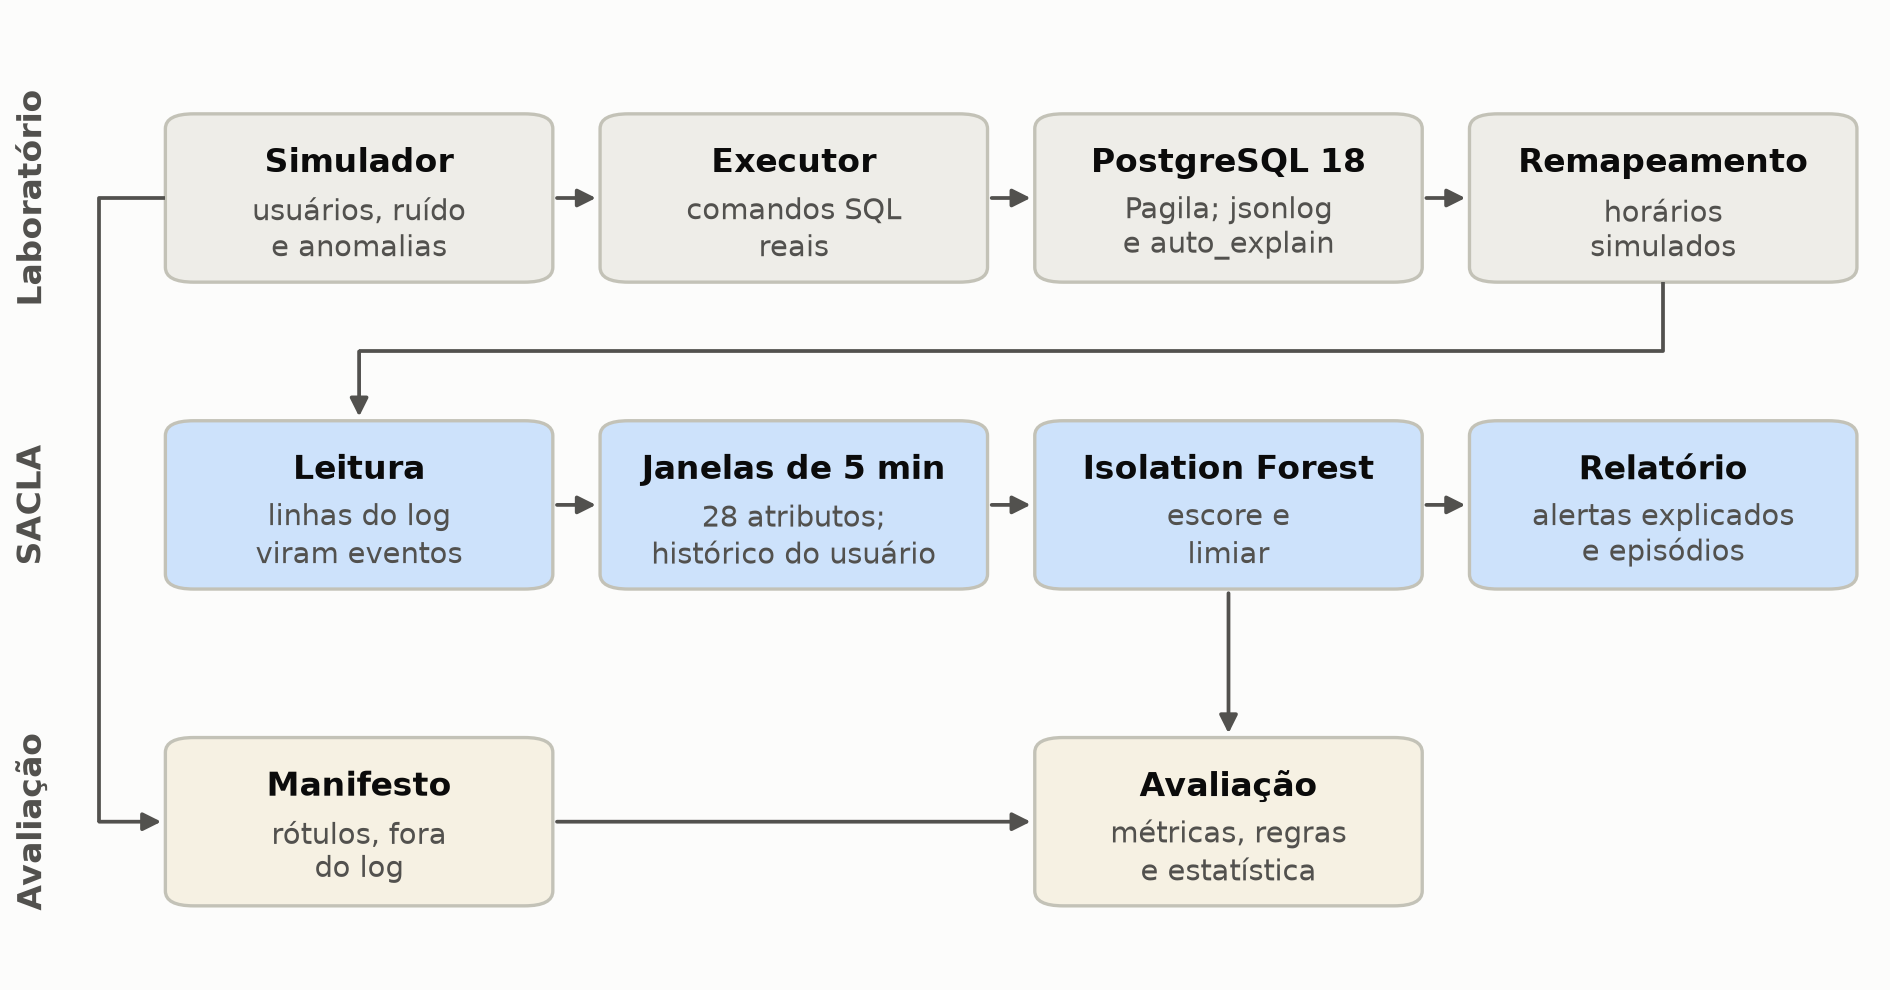
\includegraphics[width=\textwidth]{figuras/04-desenvolvimento/fluxo.png}
        \par
        \legend{Fonte: Própria do autor (2026).}
    \end{minipage}
\end{figure}

\subsubsection{Laboratório de simulação}

O laboratório tem 10 usuários em 5 papéis, cada um com privilégios mínimos concedidos por
\texttt{GRANT} (\autoref{qdr:perfis}). As ações de cada usuário chegam como um processo de
Poisson, com taxa que varia de um dia para outro, e cada ação se traduz em um ou mais comandos
SQL sorteados de um catálogo de consultas realistas sobre a Pagila. Cada usuário tem um gerador
aleatório próprio, derivado da semente da simulação e do seu nome, de modo que mudar um usuário
não altera o tráfego dos demais. A origem varia porque o contêiner que executa a simulação está
em três redes Docker (local, de aplicação e externa), e cada conexão escolhe a rede de acordo
com o perfil. Para que nenhuma anomalia fosse separável por um único atributo trivial, o tráfego
normal inclui ruído legítimo: erros de digitação, senhas digitadas errado, tentativas
ocasionais em tabelas sem permissão, hora extra, uma extração semanal grande dos analistas e a
rotina noturna volumosa do serviço \textit{batch}.

\begin{quadro}[htb]
    \centering
    \ABNTEXfontereduzida
    \begin{minipage}{\textwidth}
        \caption{\label{qdr:perfis}Papéis e rotinas dos usuários simulados}
        \begin{tabular}{|L{2.4cm}|c|L{7.6cm}|L{2.9cm}|}
            \hline
            \textbf{Papel} & \textbf{Usuários} & \textbf{Rotina} & \textbf{Origem} \\
            \hline
            atendente & 4 & turnos das 8h às 14h ou das 13h às 19h, de segunda a sábado;
            cadastro, locações e pagamentos & rede local \\
            \hline
            gerente & 2 & das 9h às 18h, de segunda a sexta, com hora extra ocasional; consultas
            amplas, alterações de cadastro e estornos & local (10\% externa) \\
            \hline
            analista & 2 & das 9h às 18h, de segunda a sexta; só leitura de dados agregados e
            relatórios & local (20\% externa) \\
            \hline
            serviço web & 1 & 24 horas, com pico às 20h; catálogo, disponibilidade e locação
            pela internet & rede de aplicação \\
            \hline
            serviço \textit{batch} & 1 & rotina diária às 2h; leituras grandes, atualização em
            lote e de uma visão materializada & rede de aplicação \\
            \hline
        \end{tabular}
        \legend{Fonte: Própria do autor (2026).}
    \end{minipage}
\end{quadro}

Foram definidos seis tipos de anomalia, cada um em três intensidades, e um sétimo tipo,
\textbf{inédito}, que só aparece no teste (\autoref{qdr:anomalias}). O tipo inédito não foi
usado para escrever as regras da linha de base nem para ajustar o modelo: representa um acesso
que não fere nenhuma permissão e não tem volume extremo em nenhum comando isolado. Em 28 dias
simulados, há 20 cenários no período de treino, simulando a contaminação que um histórico real
teria; 5 por tipo e intensidade na validação (90); e 8 por tipo e intensidade no teste (144),
mais 12 do tipo inédito.

\begin{quadro}[htb]
    \centering
    \ABNTEXfontereduzida
    \begin{minipage}{\textwidth}
        \caption{\label{qdr:anomalias}Tipos de anomalia injetados e as suas intensidades}
        \begin{tabular}{|L{3.0cm}|L{6.8cm}|L{4.8cm}|}
            \hline
            \textbf{Tipo} & \textbf{Descrição} & \textbf{Baixa / média / alta} \\
            \hline
            rajada & taxa de comandos muito acima da normal do usuário, por 3 a 8 minutos &
            3$\times$ / 8$\times$ / 20$\times$ \\
            \hline
            fora do horário & sessão em horário em que o usuário nunca trabalha &
            5 / 20 / 60 comandos \\
            \hline
            volume alto & leitura de muitas linhas & 2 mil / 10 mil linhas / tabelas inteiras \\
            \hline
            sem permissão & tentativas em tabelas sem \texttt{GRANT} & 1 a 2 / 5 / 15 tentativas \\
            \hline
            falha de autenticação & tentativas de \textit{login} com senha errada &
            3 / 10 / 40 tentativas \\
            \hline
            DML incomum & \texttt{UPDATE} ou \texttt{DELETE} permitido, em volume atípico &
            5 / 50 / 500 linhas \\
            \hline
            leitura atípica (inédito) & paginação lenta de tabelas permitidas, em horário e
            ritmo normais & 8 / 20 / 40 páginas \\
            \hline
        \end{tabular}
        \legend{Fonte: Própria do autor (2026).}
    \end{minipage}
\end{quadro}

Quatro semanas de atividade não podem ser executadas em tempo real. A agenda é gerada em tempo
simulado, os eventos são executados em sequência, em cerca de 100 segundos, e cada linha do log
recebe depois o horário simulado do seu evento, ligado a ela por um comentário opaco acrescentado
ao comando e removido no remapeamento. O log remapeado tem exatamente o formato do
\textit{jsonlog} original. Verificações automáticas acompanham cada simulação: nenhuma linha de
cliente fica sem evento, a ordem cronológica é preservada e o manifesto é coerente com o log. Na
simulação de referência, as 207.769 linhas de cliente foram remapeadas, e as contagens de linhas
dos planos coincidiram com as recebidas pelo cliente em 94.174 comparações.

\subsubsection{Arquitetura do SACLA}

O SACLA tem quatro módulos: leitura, eventos, atributos e modelo. O módulo de leitura percorre os
arquivos do \textit{jsonlog}, inclusive comprimidos, na ordem de rotação, e conta e ignora linhas
malformadas. O de eventos transforma as linhas em comandos concluídos, comandos com erro, falhas
de autenticação, conexões e desconexões, associa cada plano do \texttt{auto\_explain} ao seu
comando pela sessão e pelo texto e classifica cada comando como \texttt{SELECT},
\texttt{INSERT}, \texttt{UPDATE}, \texttt{DELETE}, DDL ou outro. O de atributos agrega os
eventos por usuário em janelas fixas de cinco minutos, alinhadas ao relógio, e calcula os 28
atributos do \autoref{qdr:atributos}. O de modelo treina o \iforest{}, define o limiar, explica
os alertas e gera o relatório.

\begin{quadro}[htb]
    \centering
    \ABNTEXfontereduzida
    \begin{minipage}{\textwidth}
        \caption{\label{qdr:atributos}Atributos calculados para cada usuário e janela de cinco
        minutos}
        \begin{tabular}{|L{4.0cm}|L{11.1cm}|}
            \hline
            \textbf{Grupo} & \textbf{Atributos} \\
            \hline
            Volume de comandos & total; por tipo (\texttt{SELECT}, \texttt{INSERT},
            \texttt{UPDATE}, \texttt{DELETE}, DDL, outros) \\
            \hline
            Erros e acesso & comandos com erro; erros de permissão; falhas de autenticação;
            conexões \\
            \hline
            Dados & linhas retornadas (soma e máximo); linhas afetadas \\
            \hline
            Desempenho & duração média, máxima e percentil 95 dos comandos \\
            \hline
            Diversidade & tabelas distintas; endereços IP distintos \\
            \hline
            Tempo & hora do dia (seno e cosseno); fim de semana \\
            \hline
            Relativos ao histórico do usuário & $z$ robusto de comandos e de linhas retornadas;
            raridade da hora; frações de tabelas, IPs e formatos de consulta nunca vistos \\
            \hline
        \end{tabular}
        \legend{Fonte: Própria do autor (2026).}
    \end{minipage}
\end{quadro}

Os seis atributos relativos tratam as anomalias contextuais, comparando a janela com o histórico
do próprio usuário $u$. O $z$ robusto de comandos de uma janela com $x$ comandos é

\begin{equation}
    z_u(x) = \frac{x - \mathrm{med}_u}{\max\left(1{,}4826 \cdot \mathrm{MAD}_u,\ 1\right)},
    \label{eq:zrobusto}
\end{equation}

\noindent em que $\mathrm{med}_u$ e $\mathrm{MAD}_u$ são a mediana e o desvio absoluto mediano
do usuário; o de linhas usa $\ln(1 + \text{linhas retornadas})$. A raridade da hora $h$ é

\begin{equation}
    r_u(h) = -\ln \frac{n_u(h) + 1}{N_u + 24},
    \label{eq:raridade}
\end{equation}

\noindent em que $n_u(h)$ é o número de janelas do histórico do usuário na hora $h$ e $N_u$ o
total, com suavização de Laplace. As frações de novidade são as frações de tabelas, de endereços
IP e de formatos de consulta (pelo \texttt{query\_id}) da janela que nunca apareceram no
histórico do usuário. O histórico usa apenas janelas do período de treino, o que é verificado por
testes automatizados, e um usuário sem histórico recebe uma referência neutra.

O modelo é o \iforest{} do scikit-learn, treinado com todas as janelas do treino, sem rótulos,
com a transformação $\ln(1+x)$ nas contagens. O escore é o oposto de \texttt{score\_samples}, de
modo que valores maiores indicam janelas mais atípicas, e uma janela gera alerta quando o escore
passa de um limiar explícito. Cada alerta é explicado pelos atributos mais raros para aquele
usuário: para cada atributo, mede-se a fração das janelas do histórico com valor maior ou igual
ao da janela, e entram até três atributos com essa fração abaixo de 5\%. O texto é escrito para
quem analisa, por exemplo ``linhas retornadas (soma): 112.507 (acima do máximo do histórico;
mediana 61, máximo 10.072)''. A explicação descreve o que mais foge do normal do usuário, e não a
atribuição interna do modelo; quando nenhum atributo isolado é raro, o alerta informa que a
combinação de valores é que é incomum. Alertas seguidos do mesmo usuário, separados por no
máximo uma janela, formam um \textbf{episódio}, que é a unidade examinada pelo analista.

%-------------------------------------------------------------------------------
% Implementação
%-------------------------------------------------------------------------------
\subsection{Implementação}
\label{sec:implementacao}

Três decisões de implementação têm efeito direto nos resultados. A primeira é o limiar. Na
avaliação, ele é o de melhor F1 na validação; no uso real, sem rótulos, é o escore acima do qual
fica uma fração fixa das janelas do próprio histórico, ou seja, o analista diz quantos alertas
aceita receber em um período normal. Na configuração avaliada, essa fração é de 2,13\%. Os
comandos \texttt{sacla fit} e \texttt{sacla score} aplicam esse fluxo a qualquer
\textit{jsonlog}, sem rótulos e sem o laboratório.

A segunda decisão é a mais importante, e veio de um defeito. Na primeira versão (v1), os
atributos relativos das janelas de treino eram calculados contra o histórico inteiro, que
incluía a própria janela. Nada no treino era ``novo'': as três frações de novidade valiam sempre
zero, e o \iforest{}, que só corta atributos que variam na amostra, as ignorava. Forçá-las a 1
em todas as janelas de teste não mudava nenhum escore. A correção foi comparar cada janela de
treino com o histórico do usuário \textbf{sem o seu dia}, o que este trabalho chama de
``deixando um dia de fora'' (\autoref{lst:fora-do-dia}). Depois dela, 83 janelas de treino
passaram a ter IP inédito, 13 formato de consulta inédito e 2 tabela inédita, e forçar cada
fração a 1 muda o escore em até 0,076. Treino e teste passaram a ter atributos relativos da
mesma natureza.

\begin{lstlisting}[language=Python, caption={Atributos relativos das janelas de treino, deixando um dia de fora}, label={lst:fora-do-dia}]
def out_of_day_relative(history, settings):
    parts = []
    for user, frame in history.groupby("user", sort=True):
        days = frame["window_start_local"].str[:10]
        for day in days.unique():
            # histórico do usuário sem o dia da janela
            others = frame[days != day]
            baselines = ({str(user): _baseline(others, settings)}
                         if len(others) else {})
            parts.append(add_relative_features(
                frame[days == day], baselines, settings))
    return pd.concat(parts).loc[history.index]
\end{lstlisting}

A terceira decisão é a separação entre o sistema e o laboratório. O pacote do SACLA não importa o
simulador nem a avaliação, e um teste de arquitetura falha se isso acontecer; os rótulos vêm só
do manifesto, e os eventos extraídos são conferidos, usuário por usuário, com o que o executor
fez. O código tem 206 testes automatizados, verificação estática de tipos e formatação
automática, e todo o experimento é reproduzível pelos comandos do Apêndice B.

%-------------------------------------------------------------------------------
% Resultados e Discussões
%-------------------------------------------------------------------------------
\subsection{Resultados e discussões}
\label{sec:resultados-e-discussoes}

Os resultados aparecem na ordem em que foram obtidos. Salvo indicação contrária, os valores
estão em porcentagem, e os do \iforest{} são a média de dez sementes do modelo.

\subsubsection{Protocolo de avaliação}

Uma janela é rotulada como anômala se algum cenário do manifesto do mesmo usuário intercepta o
seu intervalo. Os 28 dias são divididos em ordem temporal: semanas 1 e 2 para treino (9.109
janelas, 0,37\% anômalas), semana 3 para validação (4.684 janelas, 3,76\%) e semana 4 para teste
(4.662 janelas, 7,23\%). Os hiperparâmetros foram escolhidos só na validação, em uma grade de 54
combinações de número de árvores, tamanho da subamostra, fração de atributos por árvore e uso da
transformação logarítmica, cada uma com cinco sementes. A escolhida tem 200 árvores, 1.024
amostras por árvore, 50\% dos atributos e transformação logarítmica, com F1 de 61,0\% na
validação. No teste, cada uma das dez sementes do modelo usa o limiar escolhido na validação.

O \iforest{} ajustado foi comparado com três alternativas: o \textbf{IF sem rótulos}, com os
parâmetros padrão e o limiar no quantil de 99\% dos escores do treino; as \textbf{regras de
especialista}, seis regras com limiares fixados antes da avaliação e estatísticas por usuário
calculadas só no treino (três ou mais falhas de autenticação; um ou mais erros de permissão;
comandos acima de três vezes o percentil 99 do usuário; linhas retornadas acima do máximo do
usuário; linhas afetadas acima do máximo do usuário; e hora nunca vista para o usuário); e a
\textbf{combinação IF $\cup$ regras}, em que uma janela gera alerta se o modelo ou qualquer regra
a sinaliza. As regras foram escritas conhecendo os seis tipos de anomalia, o que as favorece.

\subsubsection{Teste na simulação de referência}

A \autoref{tab:teste} e a \autoref{fig:comparacao} mostram os quatro detectores na semana de
teste da simulação de referência, na versão corrigida (v2).

\begin{table}[htb]
    \centering
    \ABNTEXfontereduzida
    \setlength{\tabcolsep}{4pt}
    \begin{minipage}{\textwidth}
        \caption{\label{tab:teste}Desempenho no teste da simulação de referência}
        \begin{tabular*}{\textwidth}{@{\extracolsep{\fill}}lrrrrrrr}
            \toprule
            \textbf{Detector} & \textbf{Precisão} & \textbf{Recall} & \textbf{F1} &
            \textbf{FP} & \textbf{Cenários} & \textbf{ROC-AUC} & \textbf{PR-AUC} \\
            \midrule
            IF ajustado     & 76,5 $\pm$ 3,7 & 61,7 $\pm$ 4,3 & 68,1 $\pm$ 2,0 & 65 & 75,5 $\pm$ 4,7 & 0,953 & 0,700 \\
            IF sem rótulos  & 69,2 $\pm$ 2,3 & 27,5 $\pm$ 2,1 & 39,3 $\pm$ 2,3 & 41 & 36,3 $\pm$ 3,6 & 0,918 & 0,507 \\
            Regras          & 96,7           & 68,5           & 80,2           & 8  & 73,1           & ---   & ---   \\
            IF $\cup$ regras & 80,2 $\pm$ 3,8 & 79,3 $\pm$ 1,1 & 79,7 $\pm$ 1,3 & 67 & 86,2 $\pm$ 1,3 & ---   & ---   \\
            \bottomrule
        \end{tabular*}
        \legend{Fonte: Própria do autor (2026).}
        \legend{Nota: média $\pm$ desvio-padrão nas dez sementes do modelo; as regras são
        determinísticas. FP: falsos positivos, em janelas. A prevalência de janelas anômalas,
        7,2\%, é a PR-AUC de um detector aleatório.}
    \end{minipage}
\end{table}

\begin{figure}[htb]
    \centering
    \begin{minipage}{0.85\textwidth}
        \caption{\label{fig:comparacao}Desempenho dos detectores no teste da simulação de
        referência}
        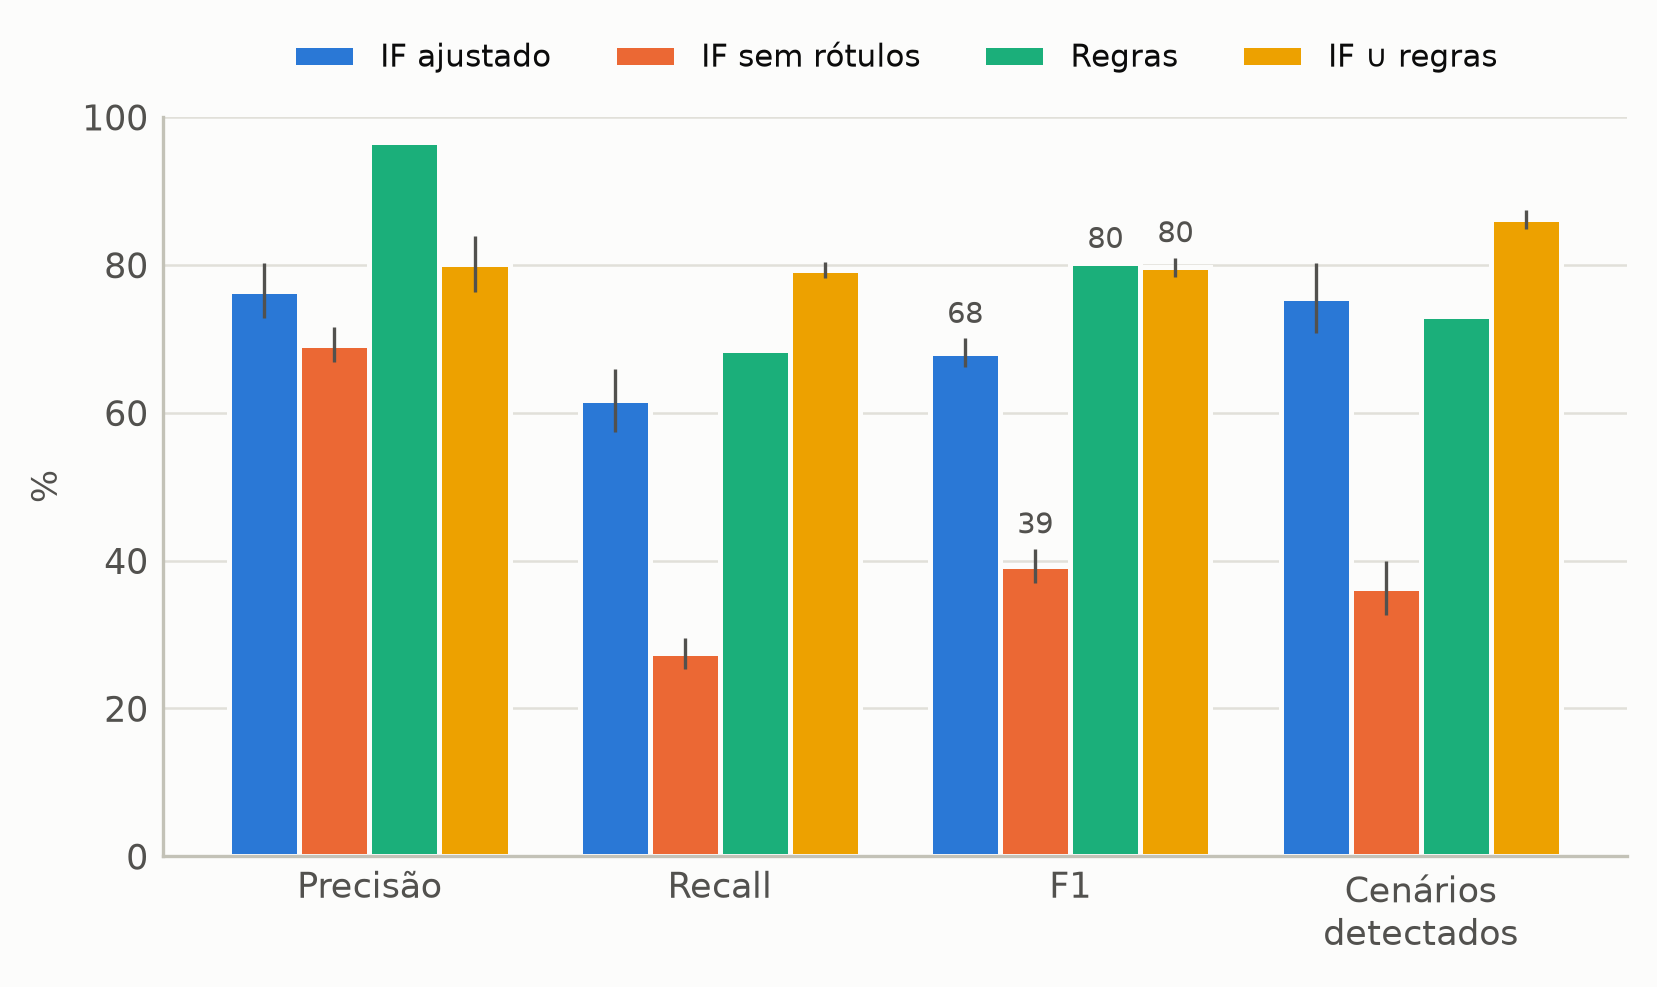
\includegraphics[width=\textwidth]{figuras/04-desenvolvimento/comparacao_detectores.png}
        \par
        \legend{Fonte: Própria do autor (2026).}
    \end{minipage}
\end{figure}

O \iforest{} ajustado obteve F1 de 68,1\%, com PR-AUC de 0,700, quase dez vezes a prevalência.
As regras tiveram F1 maior, 80,2\%, sustentado por uma precisão de 96,7\%: apenas oito falsos
positivos em toda a semana. A combinação teve F1 equivalente ao das regras, com outro perfil:
recall bem maior (79,3\% contra 68,5\%) e a maior cobertura, 86,2\% dos cenários. O IF sem
rótulos ficou bem abaixo (F1 de 39,3\%), mas não por ordenar mal as janelas, já que o ROC-AUC é
alto (0,918): sem rótulos, o limiar sinaliza poucas janelas e perde recall.

\subsubsection{Desempenho por tipo de anomalia}

A \autoref{fig:tipo-intensidade} detalha a fração de cenários detectados por tipo e
intensidade. O \iforest{} detecta bem o que é volumoso ou foge da rotina: acessos fora do
horário (91\% a 100\% dos cenários), rajadas médias e altas (82,5\% a 87,5\%) e volume alto
médio e alto (94\% a 100\%). As intensidades baixas, desenhadas para ficar na faixa do ruído
normal, são as mais difíceis; a rajada baixa, de três vezes a taxa normal, quase não é detectada
por nenhum detector. As regras são imbatíveis quando um único evento já é sinal forte, como
falhas de autenticação e erros de permissão. No tipo inédito, o \iforest{} detectou 37,5\%,
40\% e 87,5\% dos cenários de intensidade baixa, média e alta, e a combinação, de 50\% a 92,5\%.

\begin{figure}[htb]
    \centering
    \begin{minipage}{0.8\textwidth}
        \caption{\label{fig:tipo-intensidade}Cenários detectados no teste, por tipo e
        intensidade}
        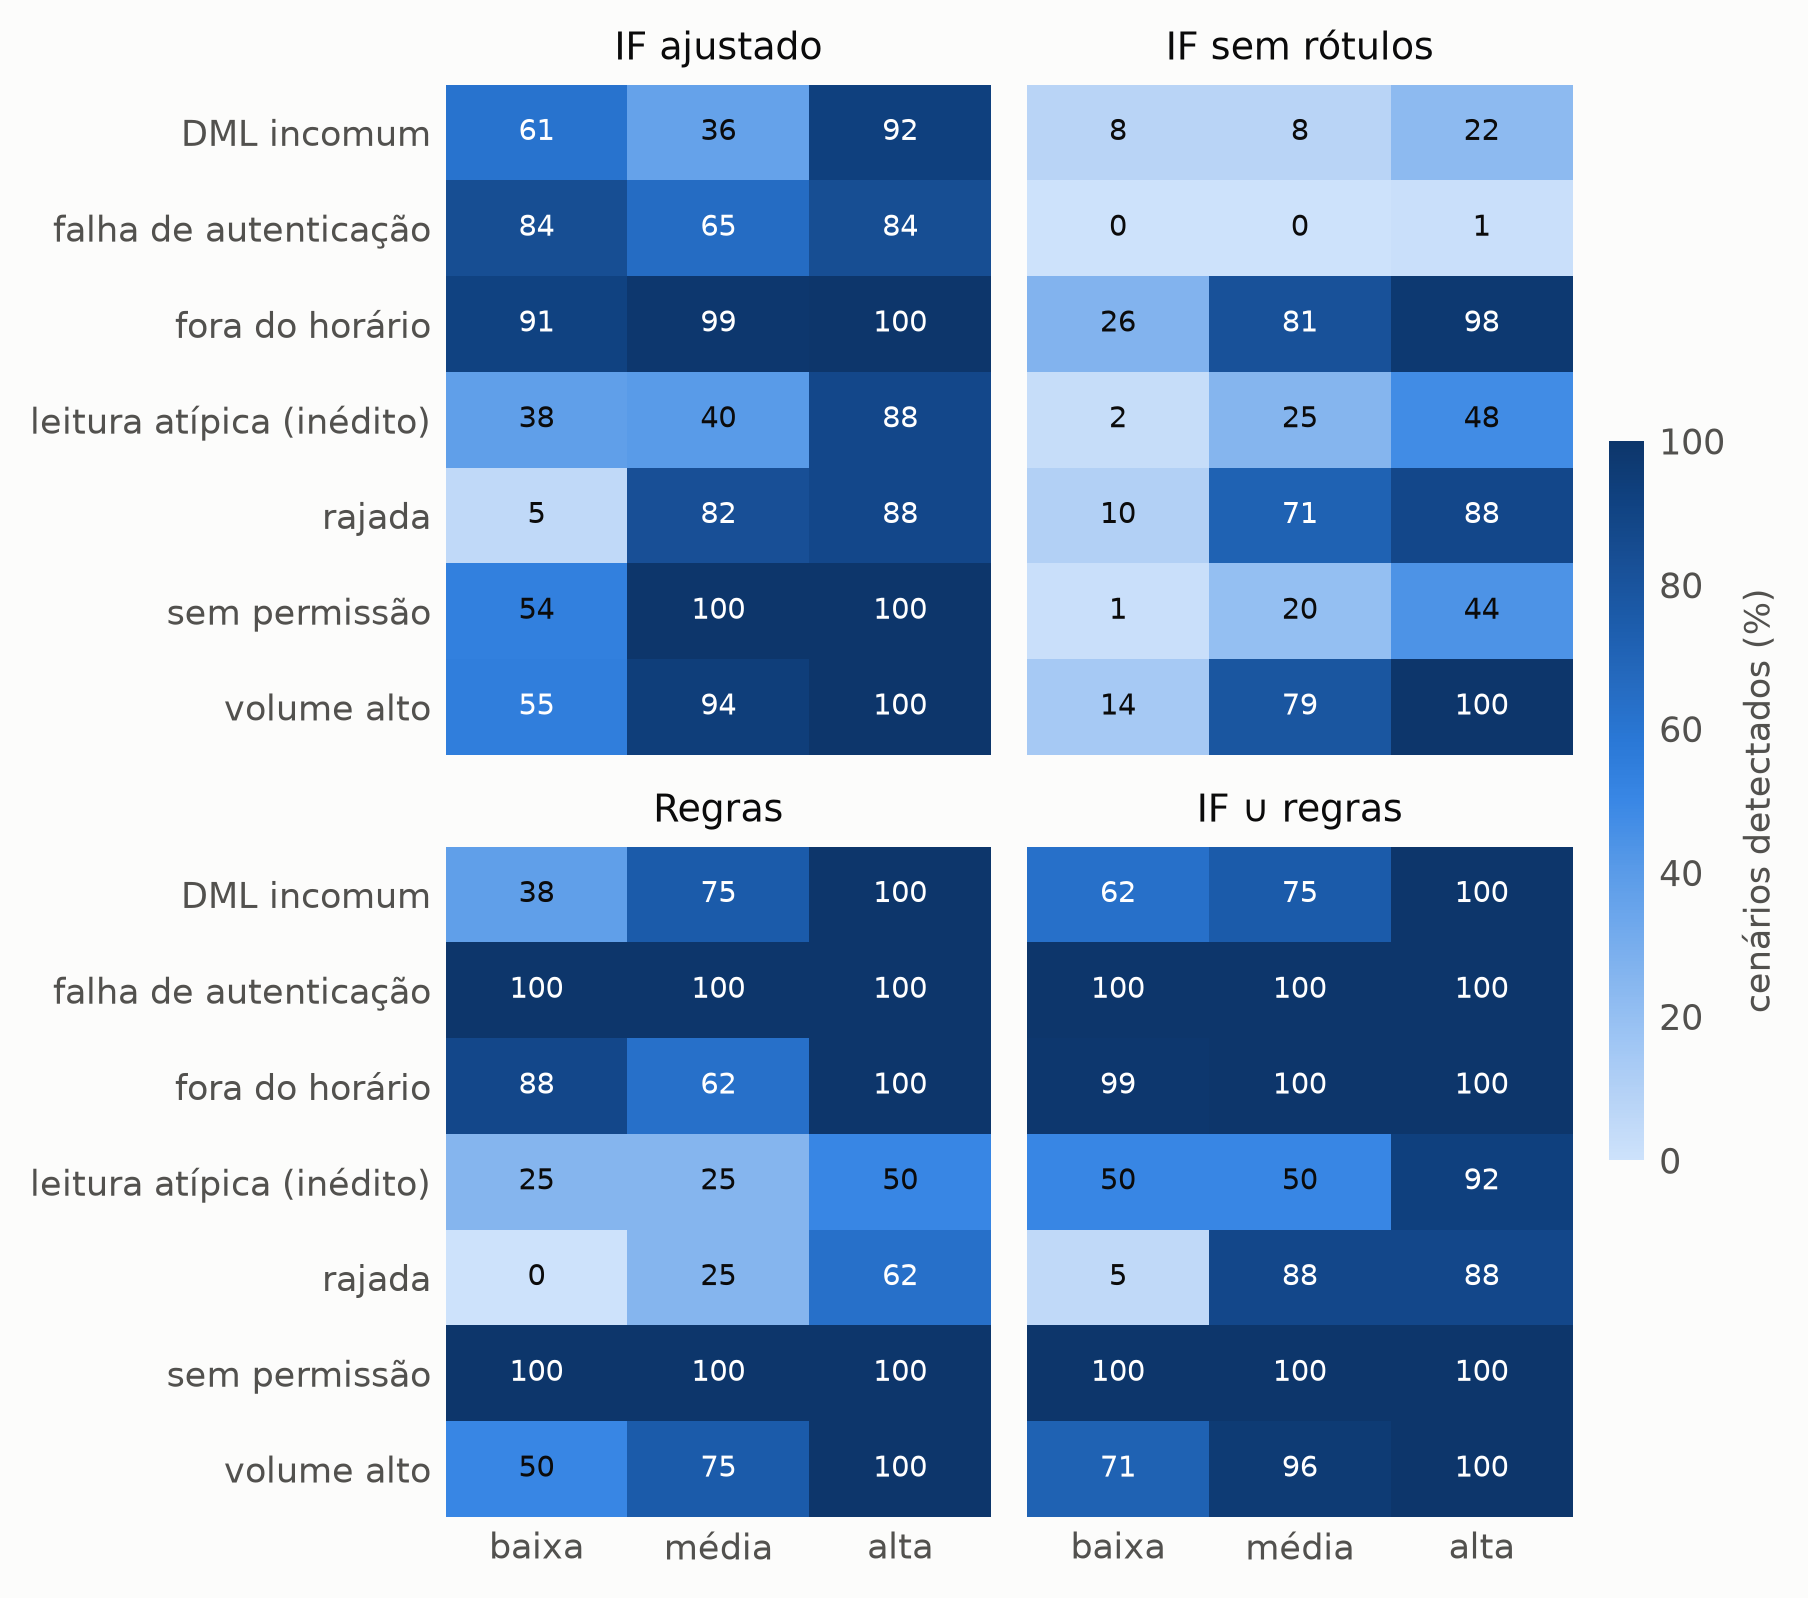
\includegraphics[width=\textwidth]{figuras/04-desenvolvimento/deteccao_tipo_intensidade.png}
        \par
        \legend{Fonte: Própria do autor (2026).}
    \end{minipage}
\end{figure}

A \autoref{fig:if-regras} classifica cada cenário de teste conforme quem o detectou. Os que só
o \iforest{} detecta concentram-se em rajadas (8), acessos fora do horário (4), volume alto (4)
e no tipo inédito (4); os que só as regras detectam, em falhas de autenticação (6), DML incomum
(4) e erros de permissão (4). Os dois detectores acertam em lugares diferentes, o que explica o
ganho da combinação. Parte da vantagem das regras vem da limitação do \iforest{} citada no
Referencial Teórico: os cortes ficam dentro da faixa de valores do treino, e uma janela com 300
comandos, quando o máximo do treino era 8, percorre as árvores como uma janela de 8 comandos.
As regras comparam diretamente com o máximo do usuário e não têm esse limite.

\begin{figure}[htb]
    \centering
    \begin{minipage}{0.9\textwidth}
        \caption{\label{fig:if-regras}Cenários de teste detectados pelo \iforest{}, pelas regras,
        por ambos ou por nenhum}
        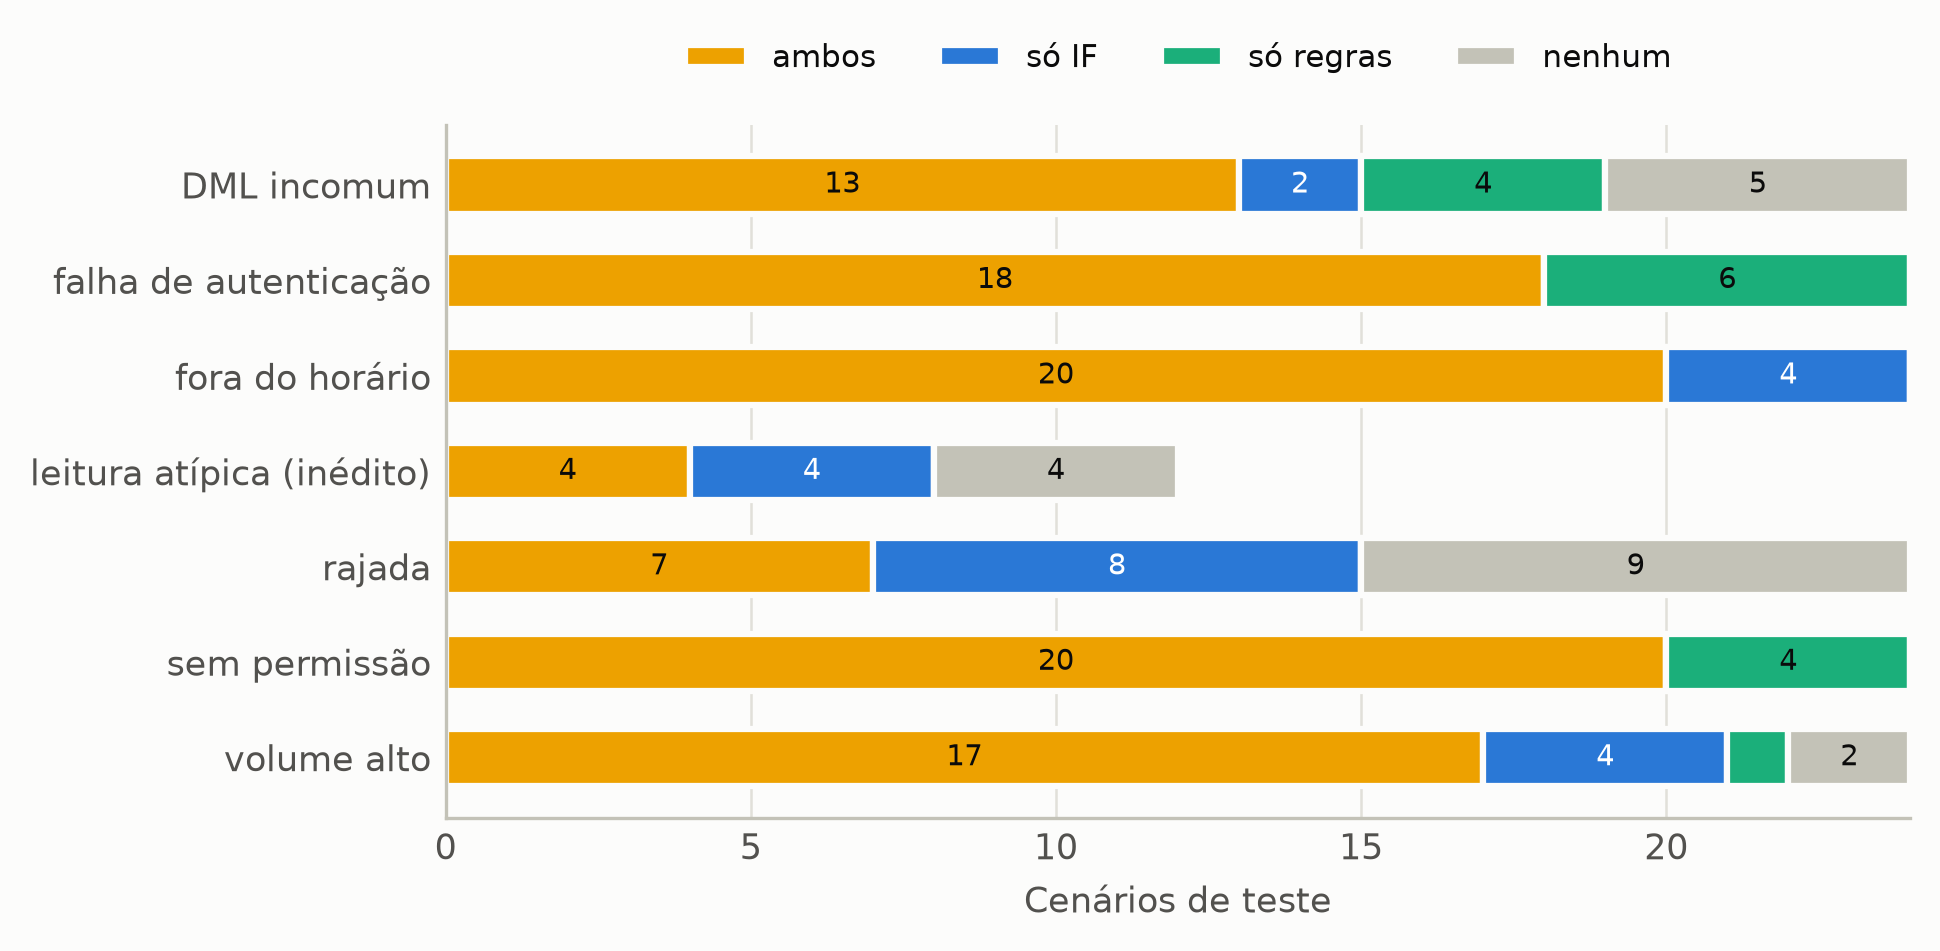
\includegraphics[width=\textwidth]{figuras/04-desenvolvimento/cenarios_if_regras.png}
        \par
        \legend{Fonte: Própria do autor (2026).}
    \end{minipage}
\end{figure}

\subsubsection{Sensibilidade, robustez, custo e a correção dos atributos}

Na validação, o resultado é estável quanto ao número de árvores e à fração de atributos por
árvore. Dois parâmetros importam: subamostras de 256 janelas reduzem o F1 de validação de 61,0\%
para 47,6\%, e não aplicar a transformação logarítmica o reduz para 56,7\%. O tamanho da janela
troca cobertura por carga de trabalho: com 1 minuto, a validação tem 82,0\% dos cenários
detectados e 422 alertas; com 5 minutos, 70,2\% e 191; com 15 minutos, 67,8\% e 106. A janela de
5 minutos foi mantida como equilíbrio. Reavaliada em duas simulações novas, com outras sementes,
a configuração congelada teve, nas três simulações, F1 de 67,2 $\pm$ 1,6 para o \iforest{} e de
78,8 $\pm$ 4,2 para as regras: o modelo depende menos da simulação. O SACLA processa as quatro
semanas de log, com 207.769 linhas de cliente, em cerca de 10 segundos (5,7~s de leitura, 3,5~s
de agregação, 0,17~s de treino e 0,6~s de relatório); o custo relevante é o do registro de log
no servidor.

A correção dos atributos relativos elevou o F1 do \iforest{} no teste de 63,8\% para 68,1\% e a
cobertura de 69,8\% para 75,5\%; nas três simulações, o F1 passou de 62,4\% para 67,2\%. O maior
ganho foi no tipo inédito de intensidade alta, de 55\% para 87,5\% dos cenários. As regras não
mudaram, porque usam só atributos absolutos e horas. O defeito foi encontrado sem olhar o
desempenho e o protocolo não mudou, mas a v2 usou o teste da simulação de referência pela
segunda vez. A validação confirmatória responde a esse uso duplo.

\subsubsection{Validação confirmatória pré-registrada}

Antes de gerar qualquer dado novo, um \textit{commit} fixou a configuração congelada, cinco
sementes de simulação nunca usadas (780 cenários de teste, 60 do tipo inédito), três hipóteses,
os testes e o nível de significância. Os testes são bicaudais, com $\alpha = 0{,}05$ e correção
de Holm, no agregado das cinco semanas de teste; um cenário conta como detectado pelo \iforest{}
quando o é em ao menos metade das dez sementes do modelo. Os intervalos de 95\% vêm de
\textit{bootstrap} percentil com 2.000 reamostragens, estratificado por simulação, com blocos
usuário--dia para as métricas por janela e cenários para a cobertura; a permutação usa os mesmos
blocos e 10.000 permutações. As simulações de desenvolvimento, reavaliadas pelo mesmo código,
reproduziram os números publicados, com diferença máxima de $5{,}6 \times 10^{-17}$.

\begin{table}[htb]
    \centering
    \ABNTEXfontereduzida
    \setlength{\tabcolsep}{3pt}
    \begin{minipage}{\textwidth}
        \caption{\label{tab:confirmatorio}Desempenho no agregado das simulações confirmatórias}
        \begin{tabular*}{\textwidth}{@{\extracolsep{\fill}}lrrrrr}
            \toprule
            \textbf{Detector} & \textbf{Precisão} & \textbf{Recall} & \textbf{F1} &
            \textbf{Cenários} & \textbf{Tipo inédito} \\
            \midrule
            IF ajustado      & 74,6 [71,4; 78,0] & 59,6 [56,2; 62,8] & 66,3 [63,4; 68,9] & 69,0 [65,9; 71,9] & 50,7 [39,3; 62,0] \\
            IF sem rótulos   & 71,7 [66,8; 76,7] & 30,9 [28,0; 34,1] & 43,2 [39,9; 46,6] & 37,5 [34,6; 40,6] & 19,3 [12,3; 26,7] \\
            Regras           & 94,7 [93,0; 96,2] & 67,9 [63,9; 71,6] & 79,1 [76,3; 81,7] & 73,5 [70,4; 76,5] & 41,7 [30,0; 53,3] \\
            IF $\cup$ regras & 78,8 [75,9; 81,6] & 79,3 [76,5; 82,1] & 79,0 [76,9; 81,2] & 84,4 [81,9; 86,7] & 76,7 [68,0; 85,3] \\
            \bottomrule
        \end{tabular*}
        \legend{Fonte: Própria do autor (2026).}
        \legend{Nota: entre colchetes, intervalo de confiança de 95\% por \textit{bootstrap}
        estratificado por simulação.}
    \end{minipage}
\end{table}

Os resultados de desenvolvimento se repetiram em dados novos (\autoref{tab:confirmatorio}): o F1
do \iforest{} foi de 66,3\%, contra 67,3\% no agregado das simulações de desenvolvimento, e a
combinação detectou 84,4\% dos cenários, contra 85,9\%. A \autoref{tab:hipoteses} reúne o
resultado das hipóteses pré-registradas, inclusive as duas do tráfego não estacionário,
apresentadas adiante, e a \autoref{fig:confirmatorio-diferencas} mostra as diferenças entre
detectores.

\begin{table}[htb]
    \centering
    \ABNTEXfontereduzida
    \setlength{\tabcolsep}{3pt}
    \begin{minipage}{\textwidth}
        \caption{\label{tab:hipoteses}Resultado das hipóteses pré-registradas}
        \begin{tabular*}{\textwidth}{@{\extracolsep{\fill}}lL{4.6cm}rrrrl}
            \toprule
            & \textbf{Medida (A $\times$ B)} & \textbf{A} & \textbf{B} &
            \textbf{A $-$ B [IC 95\%]} & \textbf{p (Holm)} & \textbf{Resultado} \\
            \midrule
            H1 & cenários detectados, IF $\cup$ regras $\times$ regras & 84,4 & 73,5 &
            +10,9 [8,9; 13,0] & $<$ 0,0001 & confirmada \\
            H2 & F1 por janela, IF $\cup$ regras $\times$ regras & 79,0 & 79,1 &
            $-$0,1 [$-$2,3; 2,5] & 1,00 & sem diferença \\
            H3 & tipo inédito detectado, IF $\times$ regras & 50,7 & 41,7 &
            +9,0 [$-$9,5; 27,0] & 1,00 & não confirmada \\
            \midrule
            H4 & perda de F1 com mudanças de rotina, IF $\times$ regras & $-$1,7 & $-$15,9 &
            +14,2 [5,8; 22,5] & 0,0039 & confirmada \\
            H5 & cenários detectados com mudanças, IF $\cup$ regras $\times$ regras & 86,1 & 74,4 &
            +11,8 [10,3; 13,3] & $<$ 0,0001 & confirmada \\
            \bottomrule
        \end{tabular*}
        \legend{Fonte: Própria do autor (2026).}
        \legend{Nota: H1 a H3 nas cinco simulações confirmatórias, com Holm sobre as três; H4 e
        H5 nas dez sementes do tráfego não estacionário, com Holm sobre as duas. H1, H3 e H5:
        McNemar exato; H2: permutação pareada por blocos; H4: $t$ pareado sobre a diferença das
        diferenças por semente.}
    \end{minipage}
\end{table}

\begin{figure}[htb]
    \centering
    \begin{minipage}{0.9\textwidth}
        \caption{\label{fig:confirmatorio-diferencas}Diferenças entre detectores no agregado
        confirmatório}
        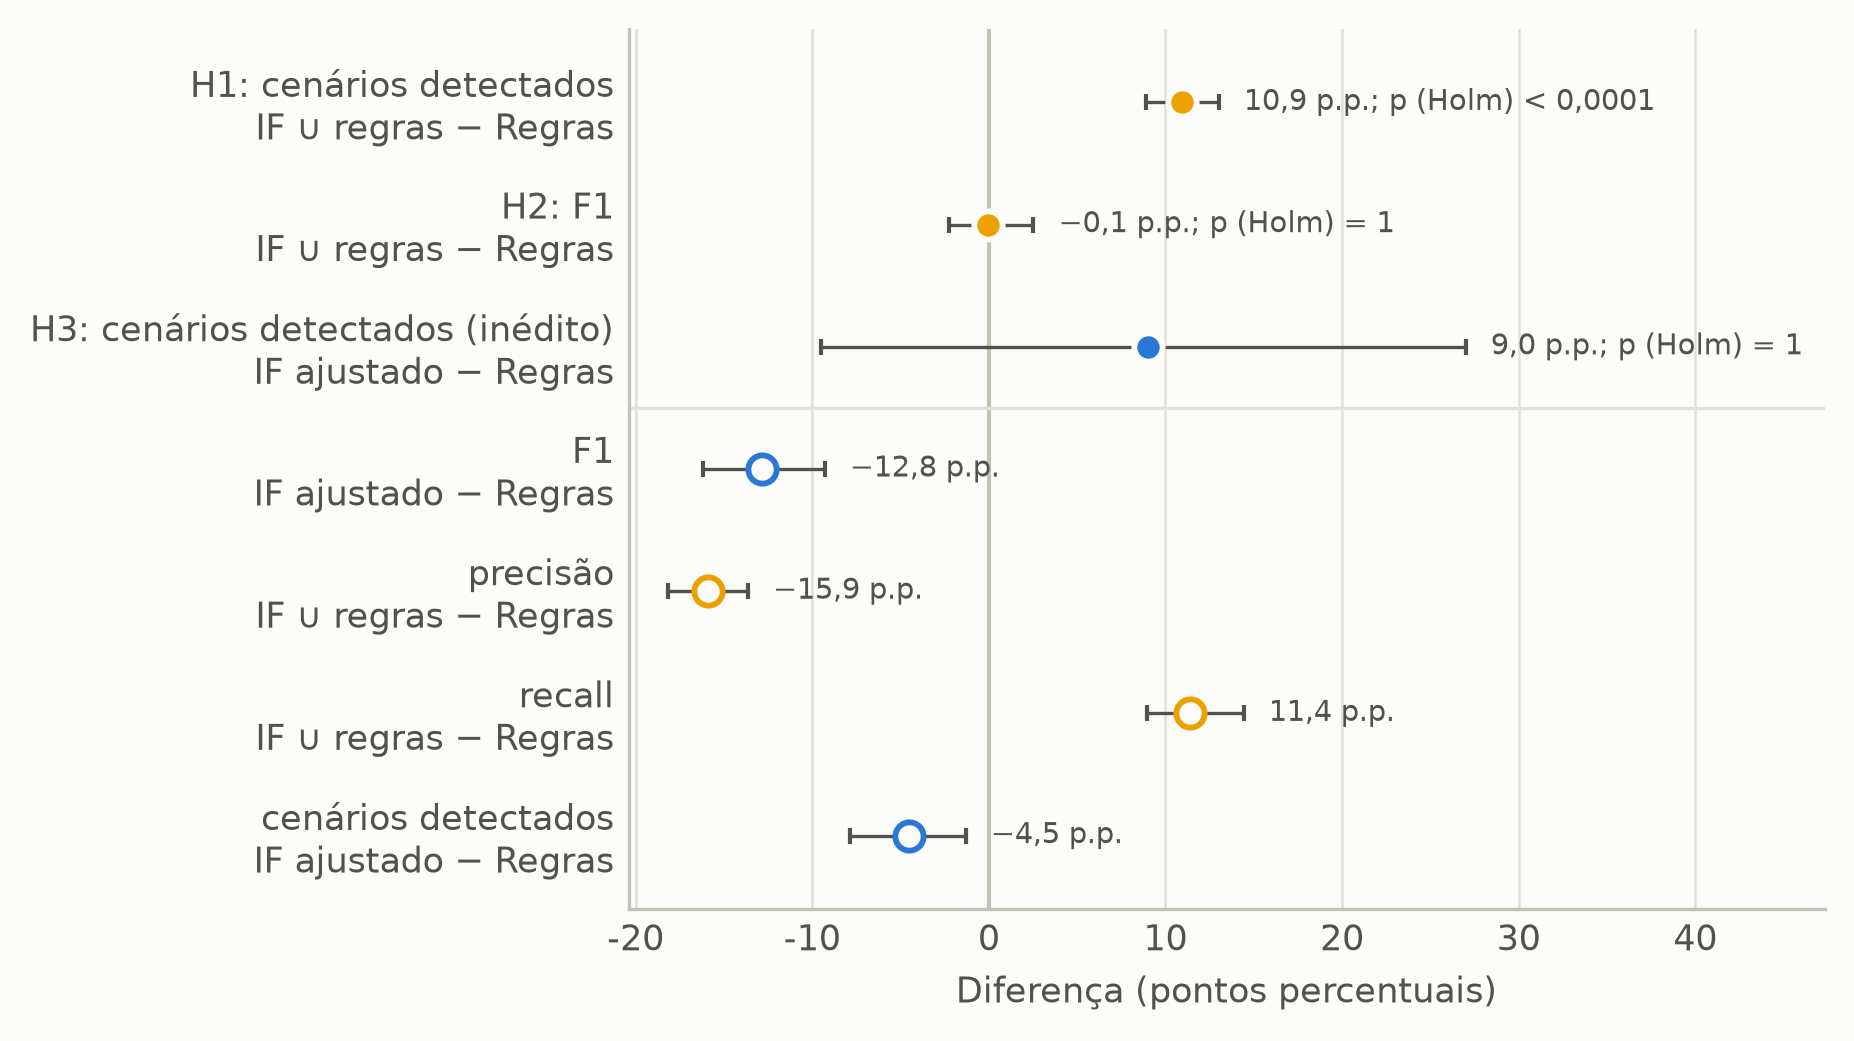
\includegraphics[width=\textwidth]{figuras/04-desenvolvimento/confirmatorio_diferencas.png}
        \par
        \legend{Fonte: Própria do autor (2026).}
        \legend{Nota: em pontos percentuais, com intervalo de 95\% por \textit{bootstrap}
        pareado. Pontos cheios: hipóteses pré-registradas, com o p ajustado por Holm; vazios:
        diferenças só descritivas.}
    \end{minipage}
\end{figure}

\textbf{H1 foi confirmada.} Em 87 dos 780 cenários, só a combinação detectou; em nenhum, só as
regras. A combinação nunca perde um cenário das regras, por construção; o teste mostra que o
ganho não é acaso, e o intervalo dá o seu tamanho, cerca de 11 pontos. \textbf{H2 não mostrou
diferença}, como esperado: a precisão cai 15,9 pontos e o recall sobe 11,4, e o F1 por janela
fica igual. Para quem faz a triagem, a escolha é entre cerca de um alerta falso a cada cinco, com
84,4\% dos cenários cobertos, e um a cada dezenove, com 73,5\%. \textbf{H3 não foi confirmada.}
No tipo inédito, os acertos se dividem: 20 cenários só o modelo detectou e 15 só as regras,
porque a regra de linhas acima do máximo do usuário detectou 25 dos 60 cenários inéditos. A
vantagem do modelo vista na simulação de referência era variação daquela simulação; o que se
sustenta é a complementaridade, já que a combinação detectou 76,7\% dos cenários inéditos.

\subsubsection{Ablação de atributos}

Para medir a contribuição de cada grupo de atributos, cada grupo foi retirado do modelo, um de
cada vez, com os hiperparâmetros congelados. A análise é exploratória e usa só o treino e a
validação das oito simulações disponíveis; o teste nunca é usado. Com todos os atributos, o F1 de
validação é de 64,9\% e a cobertura, de 73,0\% (\autoref{tab:ablacao}).

\begin{table}[htb]
    \centering
    \ABNTEXfontereduzida
    \setlength{\tabcolsep}{4pt}
    \begin{minipage}{\textwidth}
        \caption{\label{tab:ablacao}Variação ao retirar cada grupo de atributos do \iforest{}
        (validação)}
        \begin{tabular*}{\textwidth}{@{\extracolsep{\fill}}lrrrr}
            \toprule
            \textbf{Grupo retirado} & \textbf{$\Delta$ F1} & \textbf{$\Delta$ PR-AUC} &
            \textbf{$\Delta$ cenários} & \textbf{F1 pior em} \\
            \midrule
            relativos ao histórico & $-$17,0 [$-$19,4; $-$14,7] & $-$0,201 & $-$4,8 [$-$8,5; $-$1,2] & 8 de 8 \\
            horário                & $-$10,9 [$-$12,7; $-$9,1]  & $-$0,129 & $-$1,6 [$-$5,4; +2,3]  & 8 de 8 \\
            novidade               & $-$2,6 [$-$4,2; $-$1,0]    & $-$0,029 & $-$4,0 [$-$5,2; $-$2,9] & 8 de 8 \\
            origem                 & $-$0,9 [$-$2,6; +0,9]      & $-$0,012 & $-$2,2 [$-$4,8; +0,4]  & 6 de 8 \\
            dependentes do \texttt{auto\_explain} & +0,1 [$-$1,3; +1,5] & +0,017 & $-$9,6 [$-$12,7; $-$6,6] & 5 de 8 \\
            \bottomrule
        \end{tabular*}
        \legend{Fonte: Própria do autor (2026).}
        \legend{Nota: $\Delta$ = variante $-$ completo, em pontos percentuais (PR-AUC em
        unidades); entre colchetes, intervalo $t$ de 95\% entre as oito simulações.}
    \end{minipage}
\end{table}

Os atributos relativos ao histórico são o núcleo do modelo: sem eles, o F1 cai 17 pontos, em
todas as simulações, o que sustenta a decisão de comparar cada usuário consigo mesmo. O horário
vem em seguida; a novidade contribui pouco, mas sempre; e a origem não tem efeito mensurável, o
que se explica pela pouca variação que três redes simuladas produzem. Sem os atributos que
dependem do \texttt{auto\_explain}, o F1 do modelo não muda, mas a cobertura cai. No sistema
inteiro, em que as regras também perdem as duas regras de linhas, a combinação passa de 85,3\%
para 70,2\% dos cenários detectados, com a perda concentrada em volume alto (de 89,0\% para
35,5\%) e DML incomum (de 69,5\% para 32,5\%). Os cerca de 10\% de latência do
\texttt{auto\_explain} compram, portanto, cerca de 15 pontos de cobertura, justamente nos casos
de extração de dados e de alteração em massa.

\subsubsection{Tráfego não estacionário}

A principal ameaça à validade de dados sintéticos são usuários regulares demais. Um segundo
pré-registro fixou, antes de qualquer simulação, um catálogo de sete mudanças legítimas de
rotina: troca de turno, férias, pico de movimento, crescimento gradual do serviço web, trabalho
remoto (\textit{home office}), uma nova rotina de relatório em tabelas nunca usadas e um plantão
de fim de semana. O registro indicou, para cada mudança, o detector que ela deveria afetar,
inclusive algumas que só o \iforest{} enxerga. As janelas afetadas continuam rotuladas como
normais, e o plano sorteado fica em um arquivo à parte, usado só na análise. Dez sementes foram
simuladas sem e com as mudanças.

\begin{table}[htb]
    \centering
    \ABNTEXfontereduzida
    \setlength{\tabcolsep}{4pt}
    \begin{minipage}{\textwidth}
        \caption{\label{tab:deriva}Desempenho sem e com mudanças legítimas de rotina}
        \begin{tabular*}{\textwidth}{@{\extracolsep{\fill}}lrrrr}
            \toprule
            \textbf{Detector} & \textbf{F1 sem $\rightarrow$ com} & \textbf{Perda de F1 [IC 95\%]} &
            \textbf{Precisão sem $\rightarrow$ com} & \textbf{Cenários sem $\rightarrow$ com} \\
            \midrule
            IF ajustado      & 66,2 $\rightarrow$ 64,5 & $-$1,7 [$-$4,1; +0,7]   & 75,6 $\rightarrow$ 72,1 & 70,0 $\rightarrow$ 71,0 \\
            IF sem rótulos   & 41,2 $\rightarrow$ 37,8 & $-$3,4 [$-$6,8; $-$0,0] & 70,0 $\rightarrow$ 64,6 & 36,8 $\rightarrow$ 36,1 \\
            Regras           & 80,0 $\rightarrow$ 64,1 & $-$15,9 [$-$23,7; $-$8,1] & 94,0 $\rightarrow$ 61,7 & 74,7 $\rightarrow$ 74,4 \\
            IF $\cup$ regras & 79,6 $\rightarrow$ 65,3 & $-$14,2 [$-$21,5; $-$7,0] & 79,2 $\rightarrow$ 56,7 & 85,4 $\rightarrow$ 86,1 \\
            \bottomrule
        \end{tabular*}
        \legend{Fonte: Própria do autor (2026).}
        \legend{Nota: média nas dez sementes de simulação; intervalo $t$ de 95\%.}
    \end{minipage}
\end{table}

\textbf{H4 foi confirmada} (\autoref{tab:deriva}). O \iforest{} perdeu 1,7 ponto de F1, com
intervalo que inclui zero, e as regras perderam 15,9; a diferença das diferenças foi de +14,2
pontos. Com as mudanças, o F1 das regras (64,1\%) cai ao nível do \iforest{} (64,5\%).
\textbf{H5 também foi confirmada}: a combinação continua detectando cerca de 12 pontos a mais de
cenários que as regras. Nenhum detector perdeu cobertura; as mudanças geram alarmes falsos, e
não perda de detecção. A \autoref{fig:deriva-alarmes} mostra onde estão esses alarmes.

\begin{figure}[htb]
    \centering
    \begin{minipage}{0.9\textwidth}
        \caption{\label{fig:deriva-alarmes}Alarmes falsos nas janelas de teste afetadas por cada
        mudança de rotina}
        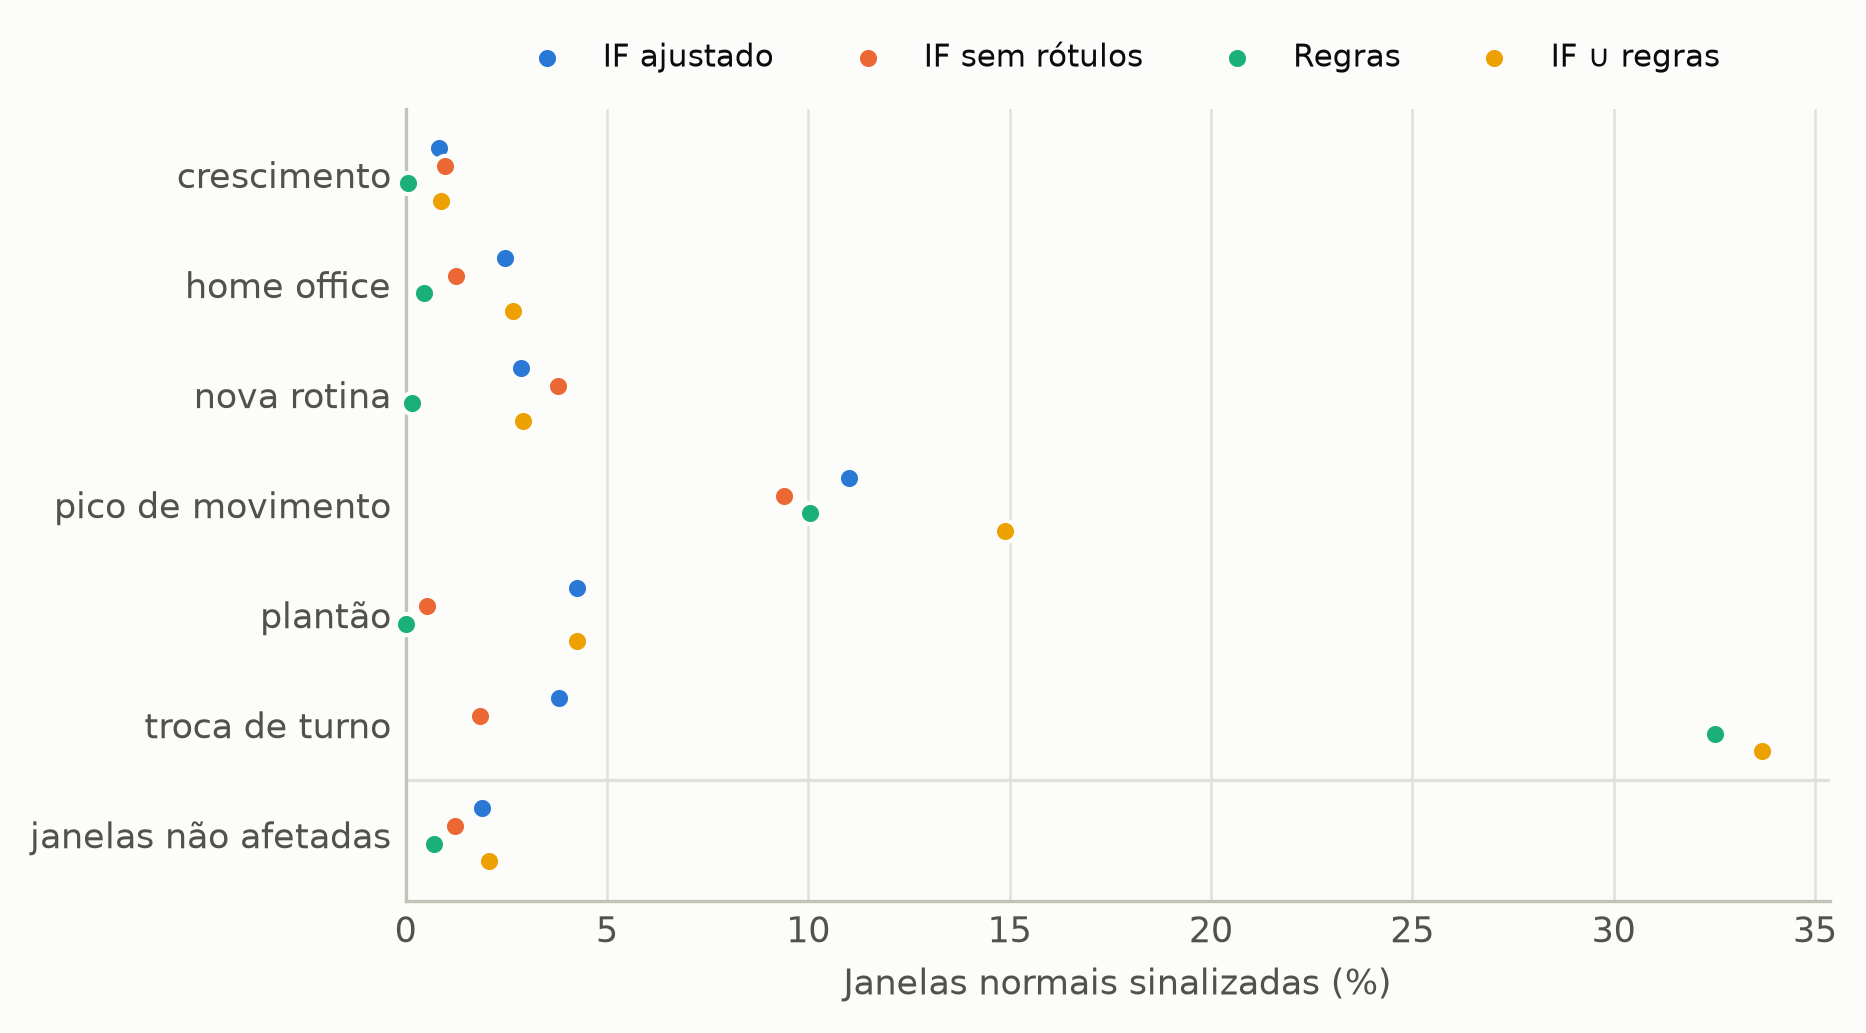
\includegraphics[width=\textwidth]{figuras/04-desenvolvimento/deriva_alarmes.png}
        \par
        \legend{Fonte: Própria do autor (2026).}
        \legend{Nota: nas férias o usuário não acessa o banco, então não há janelas afetadas.}
    \end{minipage}
\end{figure}

A perda das regras vem quase toda de uma única mudança. Na troca de turno, a regra de hora nunca
vista dispara em toda janela de um horário que o usuário não tinha no treino: 32,5\% das janelas
afetadas viram alarmes falsos, que respondem por 91\% dos alarmes falsos das regras. Nas outras
mudanças, as regras são tão ou mais robustas que o \iforest{}, abaixo de 0,5\% em crescimento,
\textit{home office}, nova rotina e plantão. O \iforest{} sofre um pouco mais nas mudanças que só
ele enxerga, como previsto no pré-registro, mas com taxas de 0,8\% a 4,3\%, próximas da sua taxa
de base de 1,9\%.

\subsubsection{Relatório explicado e ferramenta de apoio}

No teste da simulação de referência, o relatório reuniu 295 janelas sinalizadas em 195
episódios: 125 contêm ao menos uma janela de cenário anômalo, e 70 não contêm nenhuma. Os
comandos \texttt{sacla fit} e \texttt{sacla score}, aplicados aos mesmos logs, reproduziram
exatamente os escores do modelo avaliado, o que garante que o caminho de uso real é o mesmo que
foi medido. Os seis episódios de maior escore são a rotina noturna legítima do serviço
\textit{batch}, um por noite. A explicação mostra o motivo: o lote passou a ler entre 4.290 e
4.619 linhas, acima do máximo do histórico (4.014), porque as tabelas de locações e pagamentos
crescem ao longo da simulação. É uma deriva lenta dos dados, não uma anomalia de acesso, e a
explicação permite descartá-la rapidamente (\autoref{fig:relatorio}).

\begin{figure}[htb]
    \centering
    \begin{minipage}{0.62\textwidth}
        \caption{\label{fig:relatorio}Trecho do relatório de anomalias em HTML}
        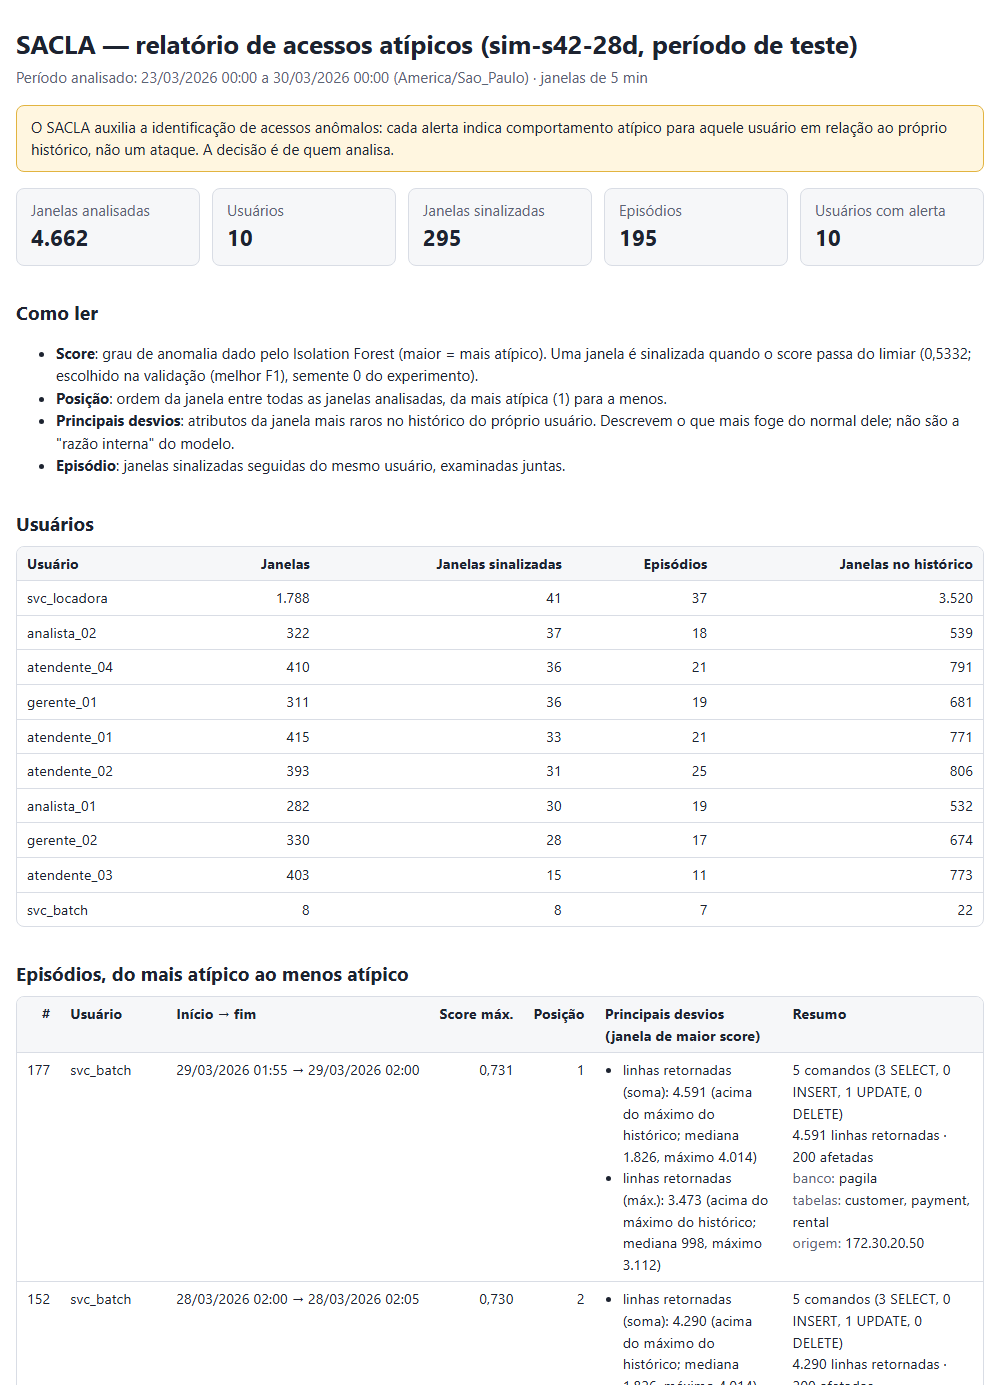
\includegraphics[width=\textwidth]{figuras/04-desenvolvimento/relatorio.png}
        \par
        \legend{Fonte: Própria do autor (2026).}
    \end{minipage}
\end{figure}

Fora da avaliação, foi construída uma ferramenta de apoio: um monitor que aplica o mesmo
detector às janelas de cinco minutos assim que elas fecham, em lotes, e um painel local,
acessível só na própria máquina, com os alertas explicados e a triagem de cada um (em análise,
suspeito confirmado ou falso positivo), mostrado na \autoref{fig:painel}. Nenhum número deste
trabalho vem dessa ferramenta, e ela não altera o modelo avaliado. Na semana de teste
reproduzida, o monitor gerou exatamente os mesmos alertas que o \texttt{sacla score} em lote:
296 janelas, uma a mais que o relatório da avaliação, porque no uso real o limiar é definido sem
rótulos.

\begin{figure}[htb]
    \centering
    \begin{minipage}{0.9\textwidth}
        \caption{\label{fig:painel}Tela de alertas do painel local}
        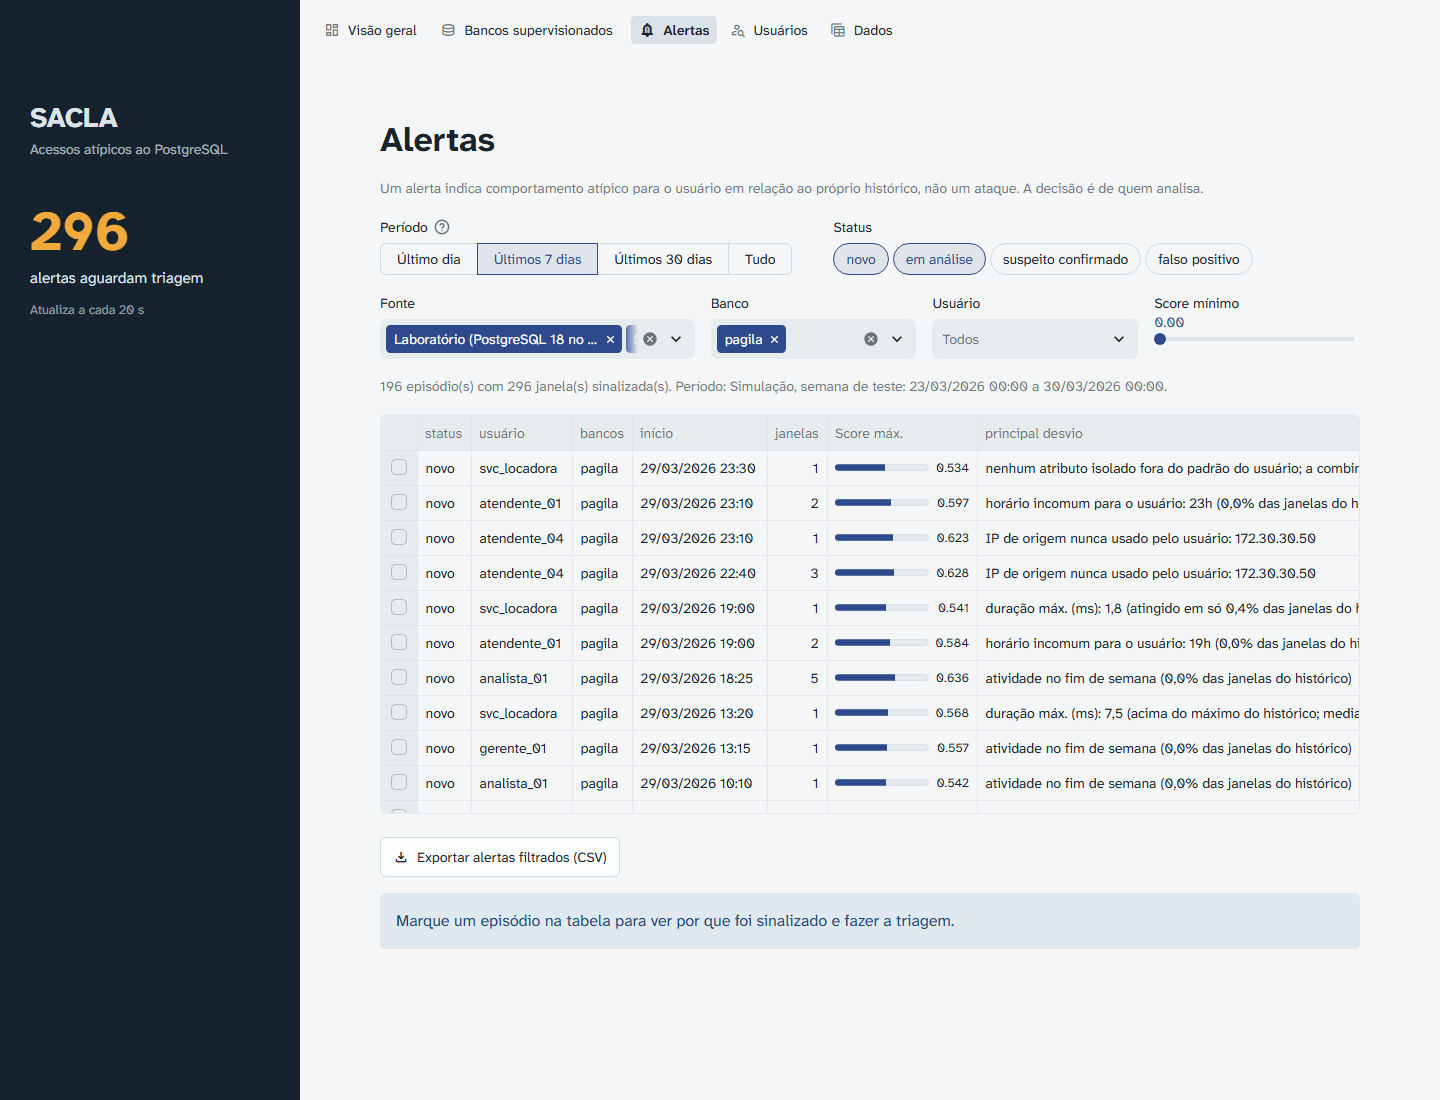
\includegraphics[width=\textwidth]{figuras/04-desenvolvimento/painel.png}
        \par
        \legend{Fonte: Própria do autor (2026).}
    \end{minipage}
\end{figure}

\subsubsection{Discussão e ameaças à validade}

Os resultados não sustentam trocar regras simples por aprendizado de máquina, e sim combinar as
duas abordagens. Regras de limiar fixo são imbatíveis para sinais inequívocos, como falhas de
autenticação em série e tentativas sem permissão: custam pouco, quase não erram e qualquer
administrador as entende. O \iforest{} acrescenta o que as regras não foram escritas para ver,
como rajadas moderadas, leituras fora do padrão e combinações incomuns de atributos, e degrada de
forma mais suave quando a rotina muda. Uma regra de ``hora nunca vista'' é razoável enquanto os
horários são estáveis e vira fonte de alarmes falsos assim que a escala muda. Em relação aos
trabalhos que modelam o papel a partir da sintaxe das consultas
\cite{kamra2008,shebaro2013,ronao2016}, o SACLA capta volume, horário, origem e falhas de
autenticação, que não aparecem no texto de uma consulta; em contrapartida, não verifica se a
consulta é típica do papel, o que esses trabalhos fazem. Os números não são diretamente
comparáveis, porque cada trabalho usa dados e anomalias próprios.

As principais ameaças à validade são as seguintes:

\begin{enumerate}[label=\alph*)]
    \item \textbf{dados sintéticos}: usuários reais variam mais, o que tende a reduzir a
          precisão de qualquer detector; o cenário com mudanças confirmou isso para as regras,
          mas o catálogo de mudanças também foi escrito pelo autor;
    \item \textbf{mesmo autor nos dois lados}: anomalias, atributos e regras foram desenhados
          pela mesma pessoa; o tipo inédito e as expectativas registradas antes dos dados
          mitigam, mas não eliminam, esse viés, que favorece as regras;
    \item \textbf{execução sequencial}: não há concorrência real entre sessões, e as durações
          são medidas sem contenção;
    \item \textbf{validade externa}: uma base pequena, um único SGBD e dez usuários;
          organizações reais têm centenas de usuários, credenciais compartilhadas por aplicações
          e padrões sazonais mais longos que quatro semanas;
    \item \textbf{validade de conclusão}: os intervalos por \textit{bootstrap} tratam as
          simulações como estratos fixos e medem a incerteza das janelas e dos cenários; a
          variação entre simulações entra no teste $t$ de H4. No tipo inédito, só 35
          discordantes não permitem distinguir uma diferença de nove pontos do acaso, e a
          ausência de significância não prova que os detectores sejam iguais.
\end{enumerate}

% ==============================================================================
% CAPÍTULO 5 - CONSIDERAÇÕES FINAIS
% ==============================================================================

\section{Considerações finais}
\label{sec:consideracoes}

Este trabalho apresentou o SACLA, um sistema que lê o log nativo do PostgreSQL e aponta, com
explicação, janelas de cinco minutos em que um usuário se comporta de forma atípica em relação
ao próprio histórico, usando um único algoritmo de aprendizado não supervisionado, o \iforest{}.
O problema de pesquisa perguntava se isso é possível com desempenho comparável ao de regras de
especialista e com alertas interpretáveis. A resposta é sim, com uma ressalva importante: o
modelo não supera as regras sozinho, mas as complementa.

Os objetivos específicos foram cumpridos. O registro de log foi configurado e o seu custo
medido, cerca de 10\% de latência mediana com o registro de linhas. O laboratório reproduz
quatro semanas de acessos de dez usuários sobre a base Pagila, com anomalias cujos rótulos
ficam fora do log. O \iforest{}, ajustado só na validação, obteve F1 de 68,1\% na simulação de
referência e de 66,3\% em cinco simulações confirmatórias nunca vistas; as regras, escritas
conhecendo os tipos de anomalia, ficaram perto de 80\%. A combinação dos dois detectou de 84\% a
86\% dos cenários, cerca de 11 pontos a mais que as regras sozinhas, o que foi confirmado com
teste estatístico em hipóteses registradas antes dos dados. Quando a rotina dos usuários muda
de forma legítima, as regras perdem 15,9 pontos de F1, quase todos por causa de trocas de turno,
e o \iforest{} perde 1,7.

As contribuições do trabalho são cinco. A primeira é um detector que usa só o log nativo, sem
extensões de auditoria nem alterações no SGBD, com o custo da instrumentação medido. A segunda
são os atributos relativos ao histórico de cada usuário, com um cuidado metodológico que se
mostrou decisivo: calcular os atributos das janelas de treino deixando um dia de fora, sem o que
as frações de novidade não têm efeito no modelo. A terceira são os alertas explicados pelos
atributos mais raros para o usuário e agrupados em episódios, o que tornou rápido descartar
alarmes falsos como o da rotina \textit{batch}. A quarta é um laboratório reprodutível, com
ruído legítimo, anomalias em três intensidades, um tipo inédito, mudanças de rotina e
verificações automáticas entre o que foi executado e o que foi registrado. A quinta é uma
avaliação com linha de base explícita, teste usado uma vez, réplicas, pré-registro, correção
para comparações múltiplas e relato dos resultados que não se confirmaram.

As principais limitações são o uso de dados sintéticos, desenhados pelo mesmo autor que escreveu
as regras e o catálogo de mudanças; uma base pequena e um único SGBD; o custo de latência do
registro de linhas; e a saturação do escore do \iforest{} para valores muito acima dos observados
no treino.

Como trabalhos futuros, o passo mais importante para a validade externa é aplicar o SACLA ao log
de um servidor em produção, mesmo sem rótulos, e analisar os alertas com quem conhece o sistema.
Outros caminhos são levar as regras para dentro do SACLA e alertar pela combinação dos dois
detectores, com as regras de horário reaprendidas após mudanças confirmadas na triagem;
reajustar o modelo periodicamente com uma janela móvel de histórico, o que trataria a deriva
lenta dos dados e as mudanças permanentes de rotina; avaliar o \texttt{auto\_explain} com
amostragem de comandos, medindo quanto de cobertura se preserva com menos custo; e acrescentar
atributos que expressem a distância de cada valor ao máximo do histórico do usuário, além de
avaliar variantes do algoritmo com cortes de inclinação aleatória, que reduzem os artefatos do
escore em regiões sem dados \cite{hariri2021}.


% ==========================================================================
% ELEMENTOS PÓS-TEXTUAIS
% ==========================================================================
\postextual

% --- Declaração sobre o uso de IA generativa (opcional) ---
% Remova ou comente a linha abaixo caso nenhuma ferramenta tenha sido utilizada.
% ==============================================================================
% DECLARAÇÃO SOBRE O USO DE IA GENERATIVA E TECNOLOGIAS ASSISTIDAS POR IA
% ==============================================================================
%
% [Conferir antes da entrega]: o texto descreve o uso do assistente de IA neste projeto.
% Ajuste a lista de finalidades se ela não corresponder ao que você fez, e acrescente a
% versão do modelo, se o curso exigir.

\section*{Declaração sobre o uso de IA generativa}
\label{sec:declaracao-uso-ia}

Durante a elaboração deste trabalho, foi utilizado o assistente Claude, desenvolvido pela
Anthropic, por meio da ferramenta Claude Code, em 2026. A ferramenta foi empregada como apoio na
implementação do código (simulador, SACLA, avaliação e testes automatizados), na execução dos
comandos do experimento, na conferência das referências e na redação de versões preliminares da
documentação e deste artigo. Todos os números relatados foram produzidos pela execução do código
versionado no repositório do projeto, e não pela ferramenta, e podem ser reproduzidos pelos
comandos do Apêndice B. Todo o conteúdo produzido com o auxílio da ferramenta foi analisado,
revisado e validado pelos autores, que assumem integral responsabilidade pelo conteúdo desta
publicação.


% --- Referências bibliográficas ---
\bibliography{referencias}
\newpage


% --- Anexos (este trabalho não tem anexos) ---

% --- Apêndices ---
\begin{apendicesenv}
    % %Imprime uma página indicando o início dos apêndices
    % \partapendices

    % ==============================================================================
% APÊNDICE A
% ==============================================================================

\section{Configuração de log do PostgreSQL}
\label{apd:apendice-a}

Configuração incluída no servidor do laboratório (arquivo \nolinkurl{docker/postgres/sacla.conf} do
repositório do projeto). A justificativa de cada parâmetro, com a documentação oficial, está em
\nolinkurl{docs/decisoes.md}.

\begin{lstlisting}[numbers=none]
# Destino e arquivos
logging_collector = on                  # obrigatório para jsonlog
log_destination = 'jsonlog'
log_directory = '/var/log/postgresql/sacla'
log_filename = 'postgresql-%Y%m%d_%H%M%S.log'
log_file_mode = 0644
log_rotation_age = 0
log_rotation_size = 100MB
log_timezone = 'UTC'

# Conexões (falhas de autenticação são registradas sempre)
log_connections = 'receipt,authentication,authorization'
log_disconnections = on

# Comandos: uma linha por comando concluído, com duração e texto
log_statement = 'none'
log_min_duration_statement = 0
log_min_error_statement = error
compute_query_id = on

# Linhas retornadas e afetadas (auto_explain)
shared_preload_libraries = 'auto_explain'
auto_explain.log_min_duration = 0
auto_explain.log_analyze = on
auto_explain.log_timing = off
auto_explain.log_buffers = off
auto_explain.log_format = 'json'
auto_explain.log_nested_statements = off
auto_explain.sample_rate = 1
auto_explain.log_level = 'LOG'
\end{lstlisting}

    \newpage
    % ==============================================================================
% APÊNDICE B
% ==============================================================================

\section{Reprodução do experimento}
\label{apd:apendice-b}

O código, a configuração e os resultados estão no repositório do projeto. Com o Docker em
execução, os comandos abaixo recriam o ambiente e reproduzem cada análise; todo o processamento
roda em contêineres com versões fixadas.

\begin{lstlisting}[numbers=none]
python tasks.py setup        # imagens, banco e Pagila do zero
python tasks.py smoke        # gera eventos conhecidos e confere o jsonlog
python tasks.py bench        # mede o custo do registro de log
python tasks.py simulate     # 28 dias simulados, semente 42
python tasks.py features     # janelas de 5 minutos, atributos e rótulos
python tasks.py evaluate     # ajuste na validação, teste, regras e sensibilidade
python tasks.py robustness --exp-id sim-s42-28d__w5m__ne200-ms1024-mf0.5-log1
python tasks.py report       # relatório de anomalias e figuras
python tasks.py confirm  --exp-id sim-s42-28d__w5m__ne200-ms1024-mf0.5-log1
python tasks.py ablation --exp-id sim-s42-28d__w5m__ne200-ms1024-mf0.5-log1
python tasks.py drift    --exp-id sim-s42-28d__w5m__ne200-ms1024-mf0.5-log1
python tasks.py test         # testes automatizados
\end{lstlisting}

Para usar o SACLA em um log real, sem rótulos, o comando \texttt{fit} aprende com um período
considerado normal, e o \texttt{score} analisa outro período e gera o relatório em HTML e CSV:

\begin{lstlisting}[numbers=none]
python tasks.py fit   --logs /logs --until 2026-03-16T03:00:00Z \
                      --model data/sacla/detector.joblib
python tasks.py score --logs /logs --since 2026-03-23T03:00:00Z \
                      --model data/sacla/detector.joblib --out data/sacla/relatorio
\end{lstlisting}

\end{apendicesenv}

% --- Índice remissivo (opcional) ---
% \phantompart
% \printindex

\end{document}
